‫
‫% -------------------------------------------------------
‫%  Abstract
‫% -------------------------------------------------------
% ‫\بدون‌تورفتگی \مهم{چکیده}: نگارش سمینار‌ علاوه بر بخش پژوهش و آماده‌سازی محتوا،
% ‫مستلزم رعایت نکات فنی و نگارشی دقیقی است 
% ‫که در تهیه‌ی یک پایان‌نامه‌ی موفق بسیار کلیدی و مؤثر است.
% ‫از آن جایی که بسیاری از نکات فنی مانند قالب کلی صفحات، شکل و اندازه‌ی قلم، صفحات عنوان و غیره در تهیه‌ی پایان‌نامه‌ها یکسان است، با استفاده از نرم‌افزار حروف‌چینی زی‌تک %\پاورقی{\XeTeX}  و افزونه‌ی زی‌پرشین %\پاورقی{XePersian}  یک قالب استاندارد برای تهیه‌ی پایان‌نامه‌ها ارائه گردیده است.
% ‫این قالب می‌تواند برای تهیه‌ی پایان‌نامه‌های کارشناسی و کارشناسی ارشد و نیز رساله‌ی دکتری مورد استفاده قرار گیرد.
% ‫این نوشتار به طور مختصر نحوه‌ی استفاده از این قالب را نشان می‌دهد.
% ‫
% ‫
% ‫%\پرش‌بلند
% ‫\بدون‌تورفتگی \مهم{واژه‌های کلیدی}: 
% ‫پایان‌نامه، حروف‌چینی، قالب، زی‌پرشین
% ‫%\صفحه‌جدید
‫
% ‫\usepackage{xepersian}
‫\settextfont{XB Niloofar} % You can replace this with any Persian font you use
‫\setlatintextfont{Times New Roman} % Set an appropriate English font
‫
‫\section{چکیده}
‫این تحقیق به بررسی و مقایسه عملکرد ابزارهای مختلف دسترسی به ذخیره‌سازی در سیستم‌های مدرن پرداخته است. در این پروژه، چهار فناوری عمده شامل \lr{libaio}، \lr{io\_uring}، و \lr{SPDK} به همراه یک شبیه‌ساز NVMe (\lr{NVMeVirt}) برای آزمایش عملکرد در پردازش‌های ورودی/خروجی (\lr{I/O}) ارزیابی شده‌اند. آزمایش‌ها با استفاده از ابزار بنچمارک \lr{FIO} انجام شده و عملکرد این فناوری‌ها در شاخص‌های مختلفی مانند IOPS (تعداد عملیات ورودی/خروجی در ثانیه)، تأخیر (\lr{Latency})، تأخیر انتهایی (\lr{Tail Latency}) و پهنای باند (\lr{Bandwidth}) بررسی گردیده است. نتایج نشان می‌دهند که هر کدام از این ابزارها بسته به نوع بار کاری و پارامترهای مختلف عملکرد متفاوتی دارند. در حالی که \lr{SPDK} به دلیل استفاده از درایورهای کاربر-محور و دور زدن کرنل، عملکرد بسیار بهتری در پردازش‌های با بار بالا دارد، \lr{libaio} در بارهای کاری با درخواست‌های تصادفی کوچک عملکرد بهتری را نشان می‌دهد. در نهایت، پیشنهاداتی برای بهینه‌سازی عملکرد و ترکیب این ابزارها برای بهبود کارایی سیستم‌های ذخیره‌سازی ارائه شده است.
‫
‫\صفحه‌جدید
‫
‫\section*{اهداف و اهمیت تحقیق}
‫هدف این تحقیق، بررسی و تحلیل عملکرد سیستم‌های ذخیره‌سازی مختلف از طریق مقایسه سه تکنولوژی مهم در دسترسی به ذخیره‌سازی یعنی \lr{libaio}، \lr{io\_uring} و \lr{SPDK} می‌باشد. استفاده از این تکنولوژی‌ها در مقایسه با روش‌های سنتی مانند فراخوان‌های سیستمی POSIX و دیگر ابزارهای مدرن می‌تواند به درک بهتری از محدودیت‌ها و پتانسیل‌های هر کدام کمک کند. این تحقیق می‌تواند راه‌حل‌های جدیدی برای بهینه‌سازی عملکرد سیستم‌های ذخیره‌سازی در مراکز داده و برنامه‌های با نیاز به کارایی بالا پیشنهاد دهد.
‫
‫در دنیای امروز، کارایی ذخیره‌سازی در بسیاری از برنامه‌ها و سیستم‌های مدرن از اهمیت ویژه‌ای برخوردار است. به ویژه در سیستم‌های پردازش داده‌های کلان و زیرساخت‌های ابری که نیاز به ذخیره‌سازی سریع و کارآمد دارند، انتخاب تکنولوژی‌های دسترسی به ذخیره‌سازی به شدت تأثیرگذار است. این تحقیق به بررسی عملکرد این تکنولوژی‌ها در موقعیت‌های مختلف پرداخته و مقایسه‌ای دقیق ارائه می‌دهد که می‌تواند راهنمایی برای انتخاب بهترین ابزار در سناریوهای مختلف باشد.
‫
‫\صفحه‌جدید
‫
‫\section{مقدمه}
‫سیستم‌های ذخیره‌سازی داده‌ها به عنوان یکی از بخش‌های حیاتی عملکرد کلی سیستم‌های رایانه‌ای محسوب می‌شوند. بهبود بهره‌وری این سیستم‌ها در سرعت خواندن و نوشتن اطلاعات از اهمیت ویژه‌ای برخوردار است. در این پروژه، ابزار \lr{NVMeVirt} مورد بررسی قرار گرفته و عملکرد آن از طریق ابزارهای \lr{FIO} و \lr{SPDK} سنجیده شده است.
‫
‫\section*{مطالعه روش‌های مختلف دسترسی به ذخیره‌سازی}
‫در سیستم‌عامل‌های مدرن، چندین روش برای دسترسی به دیسک‌های ذخیره‌سازی وجود دارد:
‫
‫\subsection*{فراخوان‌های سیستمی \lr{POSIX I/O}}
‫این روش کلاسیک، از فراخوان‌های سیستمی مانند \lr{read()} و \lr{write()} استفاده می‌کند که موجب ایجاد سربار فراخوانی سیستم و مدیریت صف‌های ورودی/خروجی در کرنل می‌شود.
‫
‫\subsection*{\lr{libaio}}
‫کتابخانه \lr{libaio} به منظور اجرای عملیات \lr{I/O} به صورت همزمان طراحی شده و باعث کاهش تأخیر ناشی از انتظار در صف‌های پردازشی کرنل می‌شود. این کتابخانه امکان مدیریت درخواست‌های ورودی/خروجی را از طریق مکانیزم \lr{event-driven} فراهم می‌کند.
‫
‫\subsection*{\lr{io\_uring}}
‫\lr{io\_uring} یکی از جدیدترین فناوری‌های بهینه‌سازی دسترسی به دیسک در سیستم‌عامل لینوکس است که با بهره‌گیری از صف‌های حلقوی \lr{ring buffer}، تعاملات ورودی/خروجی را با کمترین سربار پردازشی انجام می‌دهد.
‫
‫\subsection*{\lr{SPDK}}
‫\lr{Storage Performance Development Kit} یک مجموعه ابزار توسعه است که به منظور حذف سربار فراخوان‌های سیستمی طراحی شده و امکان برقراری ارتباط مستقیم با سخت‌افزار ذخیره‌سازی را بدون دخالت کرنل فراهم می‌کند.
‫
‫\صفحه‌جدید
‫
‫\section{شبیه‌ساز \lr{NVMeVirt}}
‫
‫\subsection*{توضیحات}
‫شبیه‌ساز \lr{NVMeVirt} یک ماژول کرنل است که یک دستگاه ذخیره‌سازی مجازی را شبیه‌سازی کرده و به عنوان یک دستگاه \lr{NVMe} برای سیستم ظاهر می‌شود. این شبیه‌ساز در سطح \lr{PCIe} پیاده‌سازی شده و امکان ارزیابی عملکرد و توسعه روش‌های بهینه‌سازی سیستم‌های ذخیره‌سازی را فراهم می‌کند.
‫
‫\subsubsection*{نحوه تعریف \lr{PCIeRoot}}
‫شبیه‌ساز \lr{NVMeVirt} در لایه \lr{PCIe} عمل می‌کند و برای تعریف آن، از مدل‌های \lr{PCIeRoot} موجود در کرنل لینوکس استفاده می‌شود. این شبیه‌سازی در لایه \lr{bus} انجام شده و به‌عنوان یک دستگاه مجازی به سیستم‌عامل معرفی می‌شود.
‫
‫\subsubsection*{مطالعه کدهای مربوطه و تهیه مستندات}
‫کد منبع \lr{NVMeVirt} شامل چندین فایل کلیدی است که نحوه ارتباط آن با سیستم را مشخص می‌کنند:
‫\begin{itemize}
‫	\item \texttt{pci.c}: مدیریت ارتباط \lr{PCIe} و پیاده‌سازی شبیه‌سازی دستگاه \lr{NVMe}.
‫	\item \texttt{nvmev.h}: شامل تعاریف کلی و پارامترهای کنترلی ماژول.
‫	\item \texttt{main.c}: شامل بخش اصلی پیاده‌سازی پردازش ورودی/خروجی و مدیریت حافظه.
‫\end{itemize}
‫
‫\subsubsection*{نحوه کارکرد شبیه‌ساز}
‫شبیه‌ساز \lr{NVMeVirt} یک ماژول کرنل است که از مکانیزم‌های مدیریت حافظه برای اختصاص فضای فیزیکی به عنوان فضای ذخیره‌سازی شبیه‌سازی شده استفاده می‌کند. این ماژول درخواست‌های ورودی/خروجی را پردازش کرده و آن‌ها را در حافظه اصلی نگهداری می‌کند.
‫
‫\subsubsection*{معماری و بخش‌های اساسی}
‫معماری \lr{NVMeVirt} از بخش‌های زیر تشکیل شده است:
‫\begin{itemize}
‫	\item \textbf{مدیریت حافظه}: اختصاص و مدیریت فضای حافظه برای شبیه‌سازی دستگاه ذخیره‌سازی.
‫	\item \textbf{مدیریت \lr{PCIe}}: ارتباط با زیرسیستم \lr{PCIe} و شبیه‌سازی دستورات \lr{NVMe}.
‫	\item \textbf{مدیریت صف‌های ورودی/خروجی}: پردازش درخواست‌های \lr{I/O} و اجرای آن‌ها به صورت شبیه‌سازی شده.
‫\end{itemize}
‫
‫\subsubsection*{سطح شبیه‌سازی}
‫شبیه‌ساز \lr{NVMeVirt} در سطح \lr{PCIe} عمل می‌کند و به‌عنوان یک دیسک مجازی \lr{NVMe} در سیستم شناخته می‌شود. این شبیه‌ساز از حافظه فیزیکی سیستم برای ذخیره داده‌ها استفاده کرده و امکان تعامل مستقیم برنامه‌های کاربر و کرنل را فراهم می‌کند.
‫
‫\subsubsection*{مکان ذخیره‌سازی داده‌ها}
‫داده‌های ذخیره‌شده توسط \lr{NVMeVirt} در حافظه اصلی قرار می‌گیرند و از طریق پارامترهای \texttt{memmap\_start} و \texttt{memmap\_size} قابل تنظیم هستند. این روش باعث افزایش سرعت دسترسی به داده‌ها می‌شود اما ممکن است میزان حافظه موجود در سیستم را کاهش دهد.
‫
‫\subsubsection*{کنترل سرعت دسترسی و شبیه‌سازی دیسک سرعت بالا}
‫برای شبیه‌سازی یک دستگاه ذخیره‌سازی پرسرعت بر روی سیستمی با دیسک کندتر، می‌توان از تنظیمات نرخ ورودی/خروجی استفاده کرد. این امر با تغییر اندازه \lr{queue depth} و استفاده از برنامه‌های آزمون مانند \lr{FIO} امکان‌پذیر است.
‫
‫‫\subsection*{مراحل نصب و شبیه سازی}
‫
‫\begin{figure}[H]
‫	‫    \centering
‫	‫    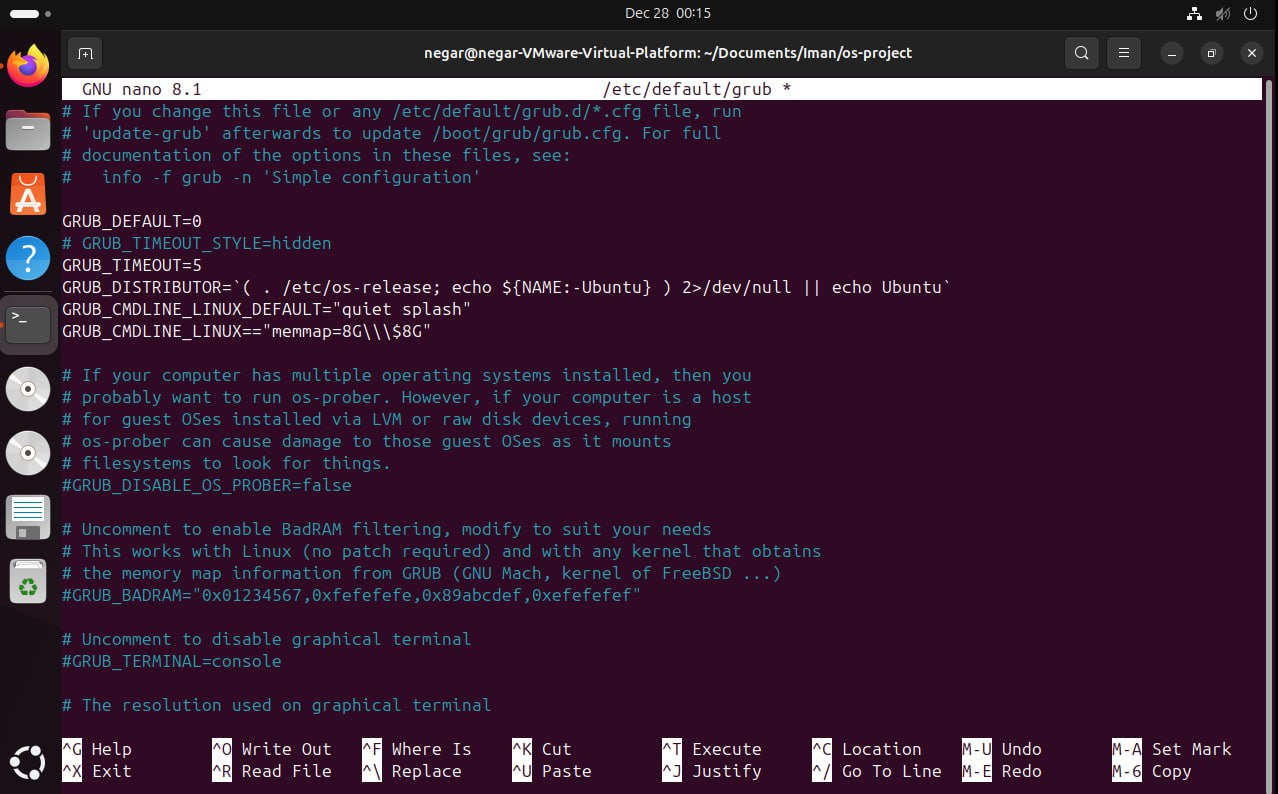
\includegraphics[width=\textwidth]{figs/11.jpg}
‫	‫    \caption{GRUB}
‫\end{figure}
‫
‫‫\begin{figure}[H]
‫	‫	‫    \centering
‫	‫	‫    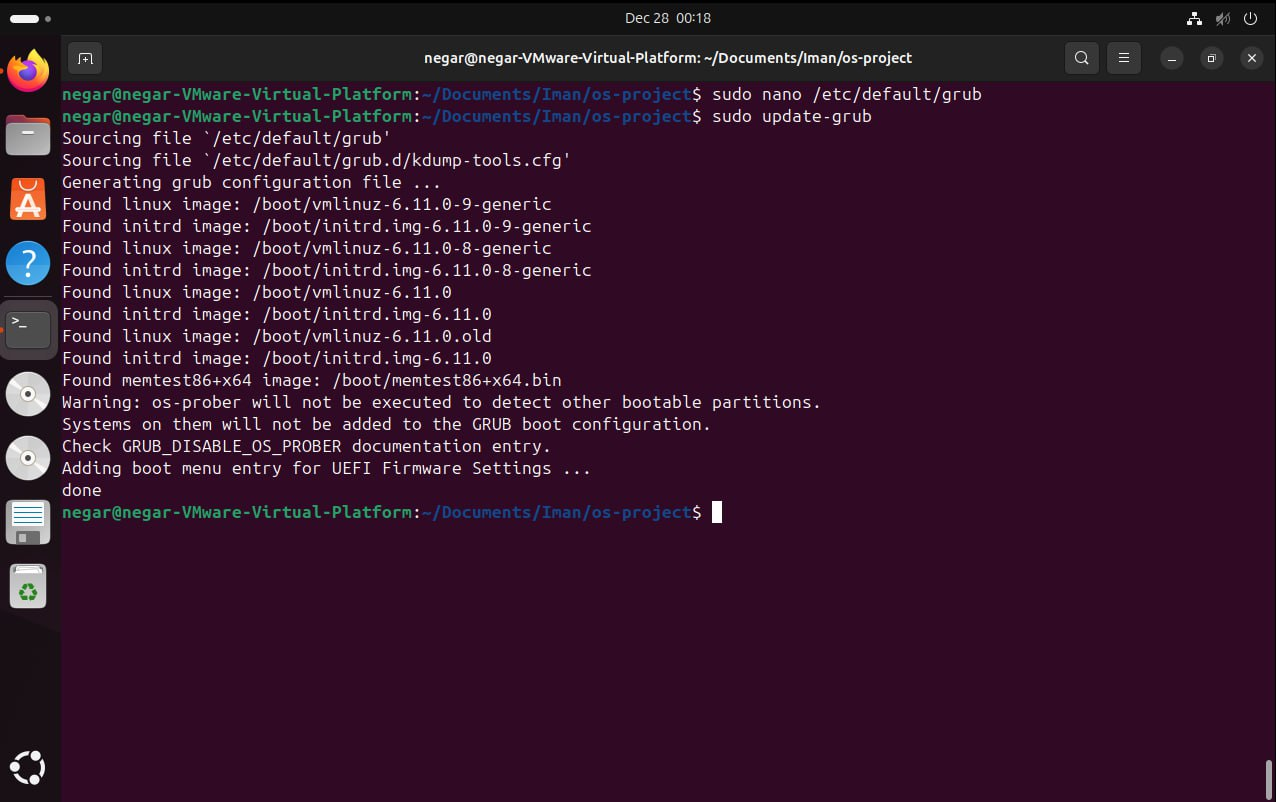
\includegraphics[width=\textwidth]{figs/12.jpg}
‫	‫	‫    \caption{آپدیت GRUB و در ادامه، ریبوت}
‫\end{figure}
‫
‫‫‫\begin{figure}[H]
‫	‫	‫	‫    \centering
‫	‫	‫	‫    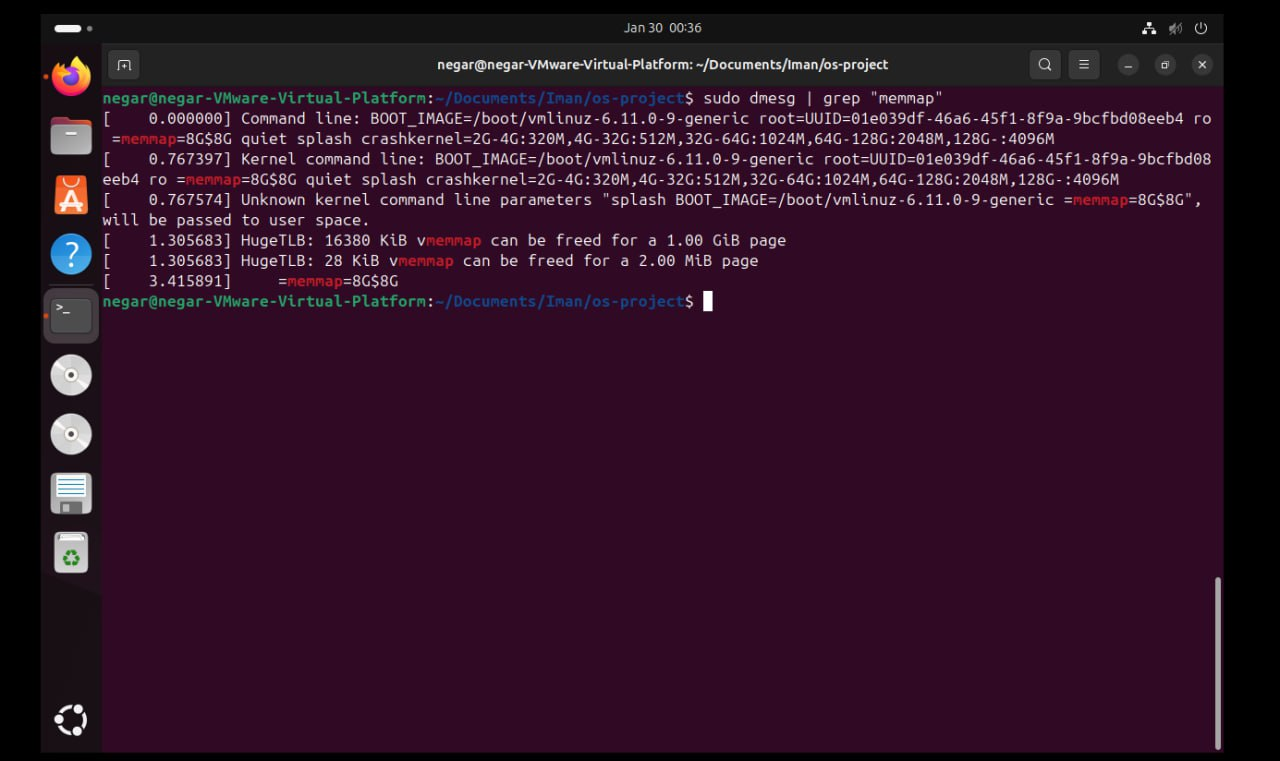
\includegraphics[width=\textwidth]{figs/13.jpg}
‫			\caption{بررسی تغییرات انجام شده}
‫\end{figure}
‫
‫\begin{figure}[H]
‫	‫    \centering
‫	‫    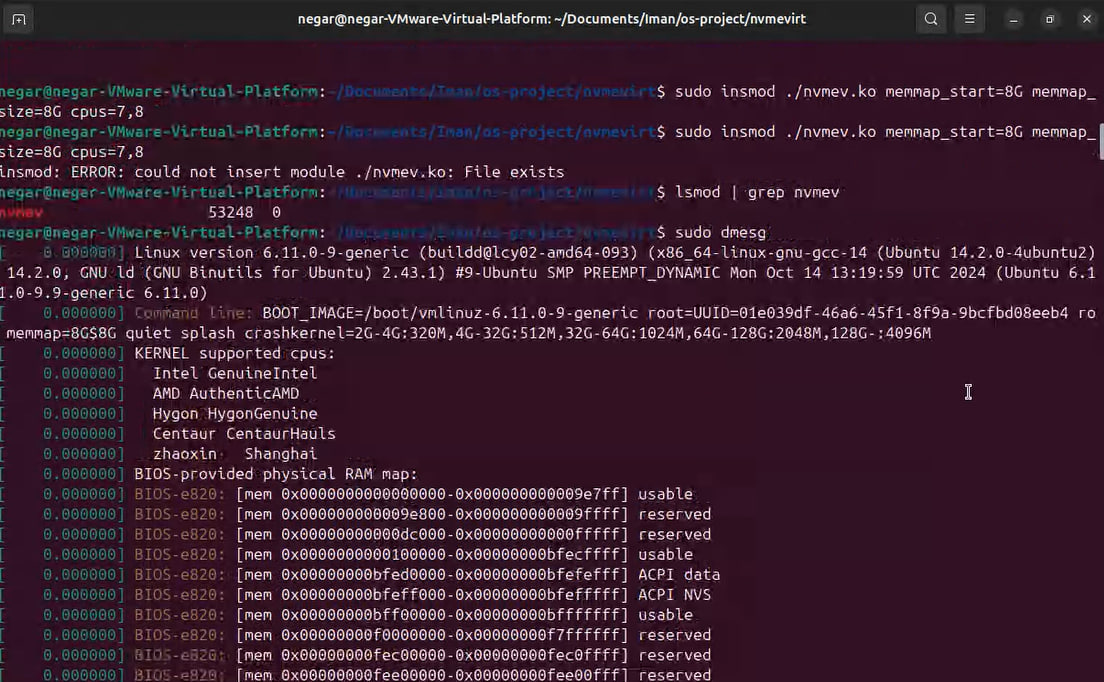
\includegraphics[width=\textwidth]{figs/14.jpg}
‫	‫    \caption{بارگذاری ماژول}
‫\end{figure}
‫
‫\begin{figure}[H]
‫	‫    \centering
‫	‫    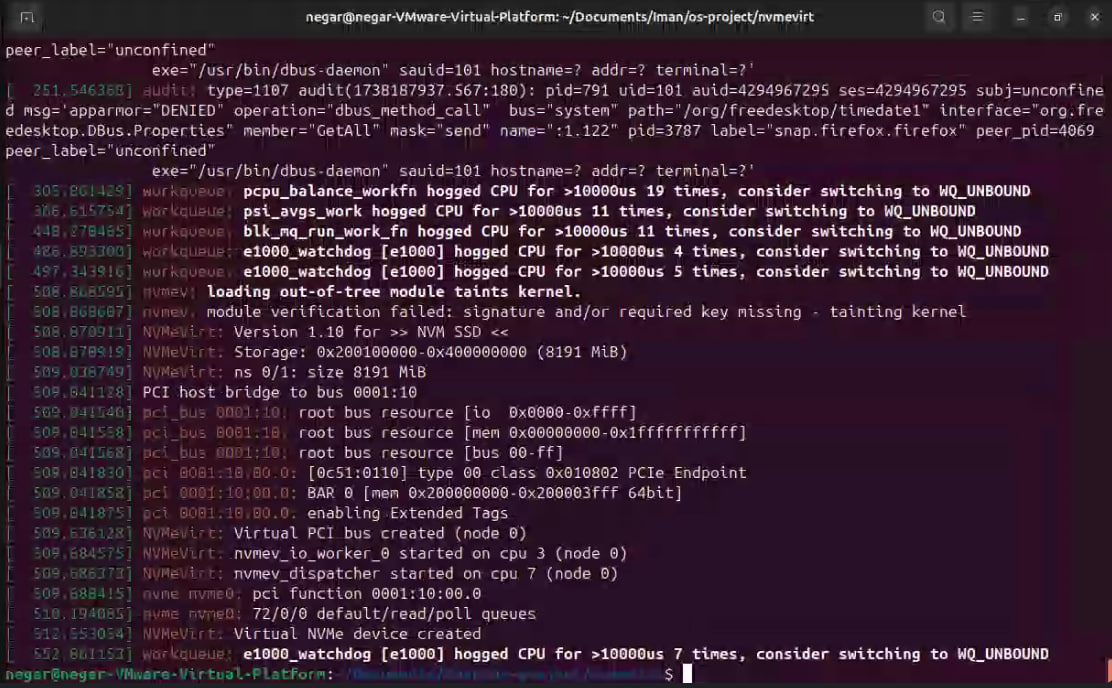
\includegraphics[width=\textwidth]{figs/15.jpg}
‫	‫    \caption{بررسی تنظیمات memmap در کرنل}
‫\end{figure}
‫
‫‫‫\begin{figure}[H]
‫	‫	‫	‫    \centering
‫	‫	‫	‫    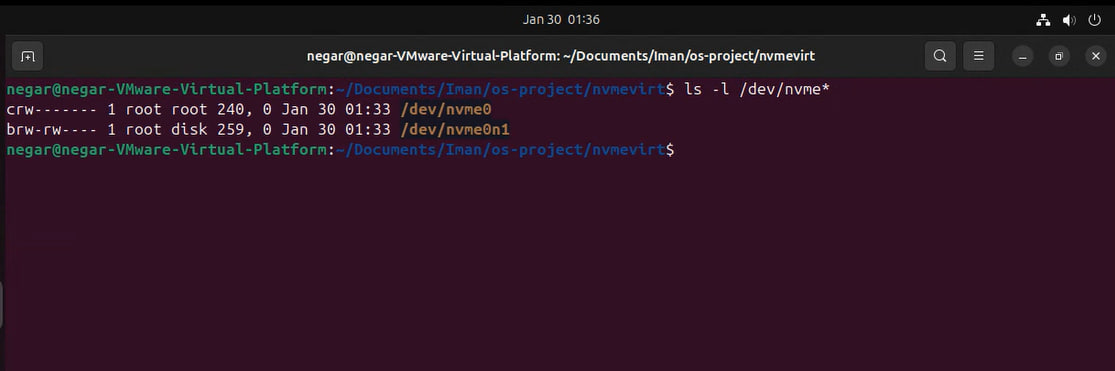
\includegraphics[width=\textwidth]{figs/16.jpg}
‫			\caption{بررسی دقیق شناسایی درست دیسک مجازی}
‫\end{figure}
‫
‫‫‫\begin{figure}[H]
‫	‫	‫	‫    \centering
‫	‫	‫	‫    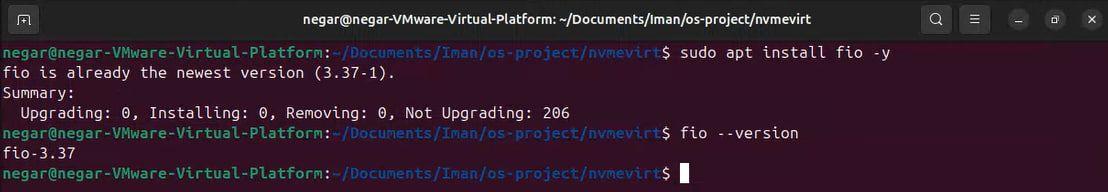
\includegraphics[width=\textwidth]{figs/17.jpg}
‫			\caption{نصب fio}
‫\end{figure}
‫
‫‫‫\begin{figure}[H]
‫	‫	‫	‫    \centering
‫	‫	‫	‫    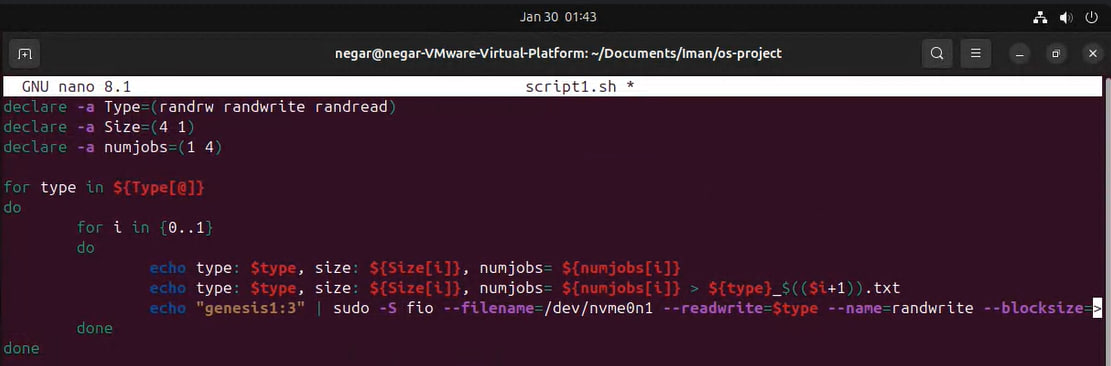
\includegraphics[width=\textwidth]{figs/18.jpg}
‫			\caption{اسکریپت تحلیل libaio}
‫\end{figure}
‫
‫‫‫\begin{figure}[H]
‫	‫	‫	‫    \centering
‫	‫	‫	‫    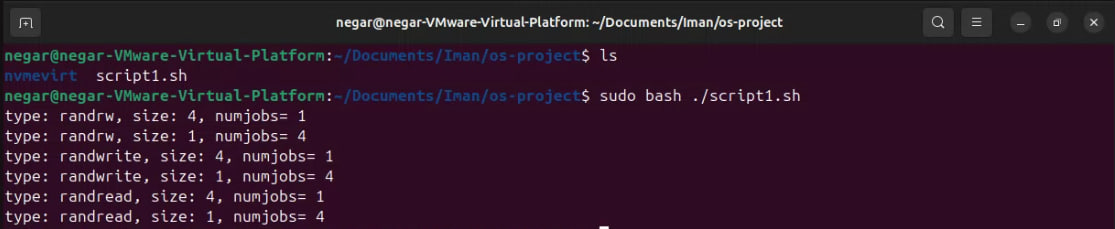
\includegraphics[width=\textwidth]{figs/19.jpg}
‫			\caption{نتیجه‌ی ران اسکریپت تحلیل libaio}
‫\end{figure}
‫
‫‫‫\begin{figure}[H]
‫	‫	‫	‫    \centering
‫	‫	‫	‫    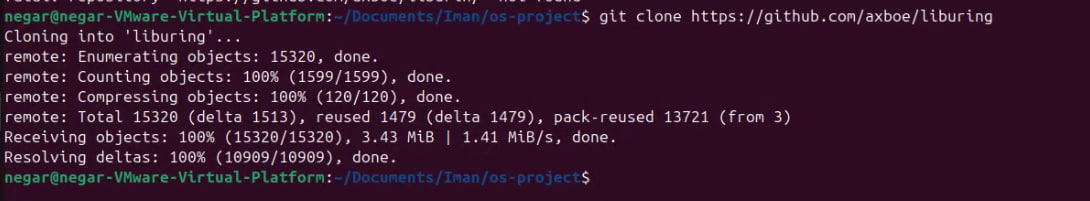
\includegraphics[width=\textwidth]{figs/20.jpg}
‫			\caption{کلون گرفتن از ریپوی liburing}
‫\end{figure}
‫
‫‫‫\begin{figure}[H]
‫	‫	‫	‫    \centering
‫	‫	‫	‫    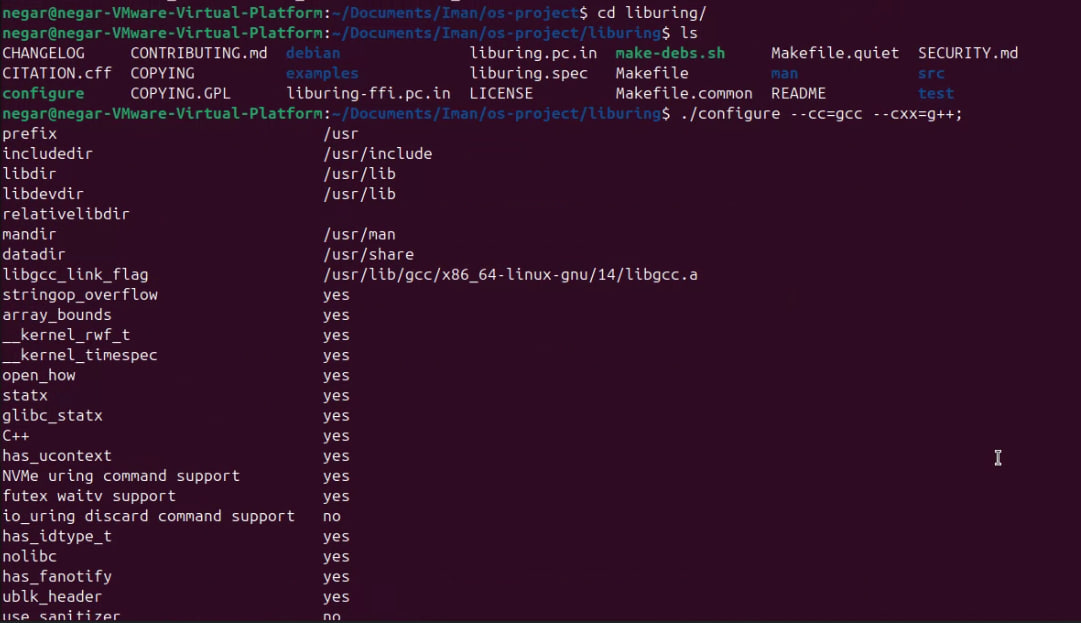
\includegraphics[width=\textwidth]{figs/21.jpg}
‫			\caption{کانفیگ liburing}
‫\end{figure}
‫
‫‫‫\begin{figure}[H]
‫	‫	‫	‫    \centering
‫	‫	‫	‫    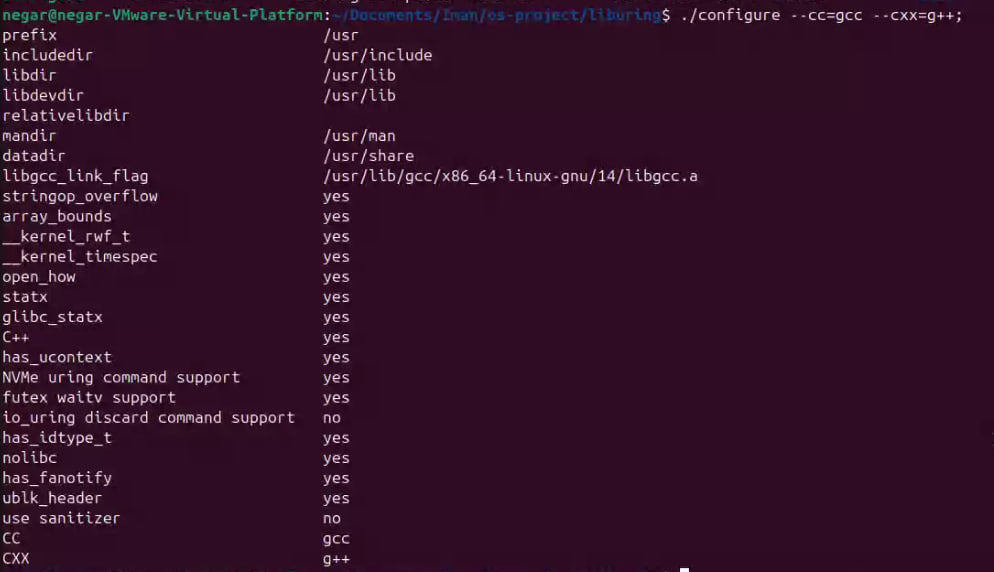
\includegraphics[width=\textwidth]{figs/22.jpg}
‫			\caption{ادامه‌ی کانفیگ liburing}
‫\end{figure}
‫
‫‫‫\begin{figure}[H]
‫	‫	‫	‫	‫    \centering
‫	‫	‫	‫	‫    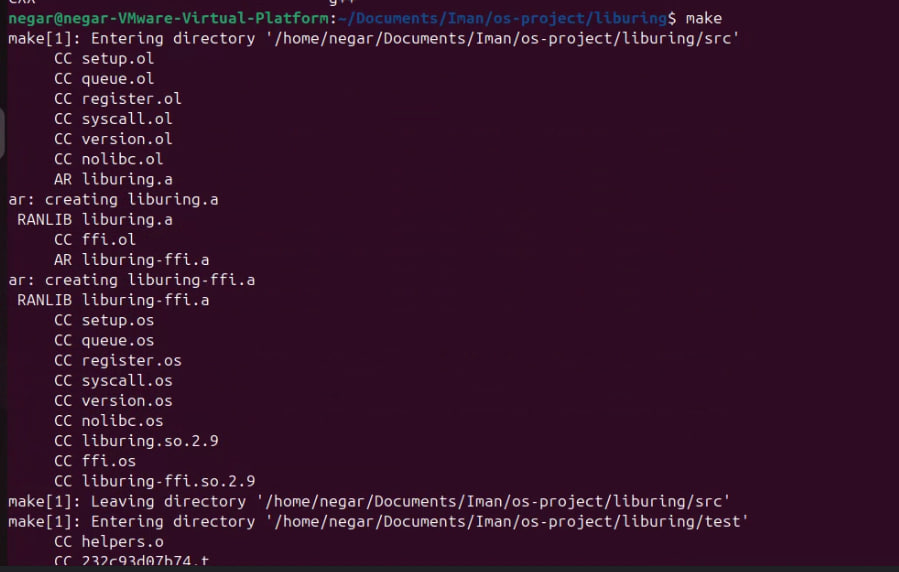
\includegraphics[width=\textwidth]{figs/23.jpg}
‫	‫			\caption{کامپایل و نصب liburing}
‫‫\end{figure}
‫
‫‫‫\begin{figure}[H]
‫	‫	‫	‫	‫    \centering
‫	‫	‫	‫	‫    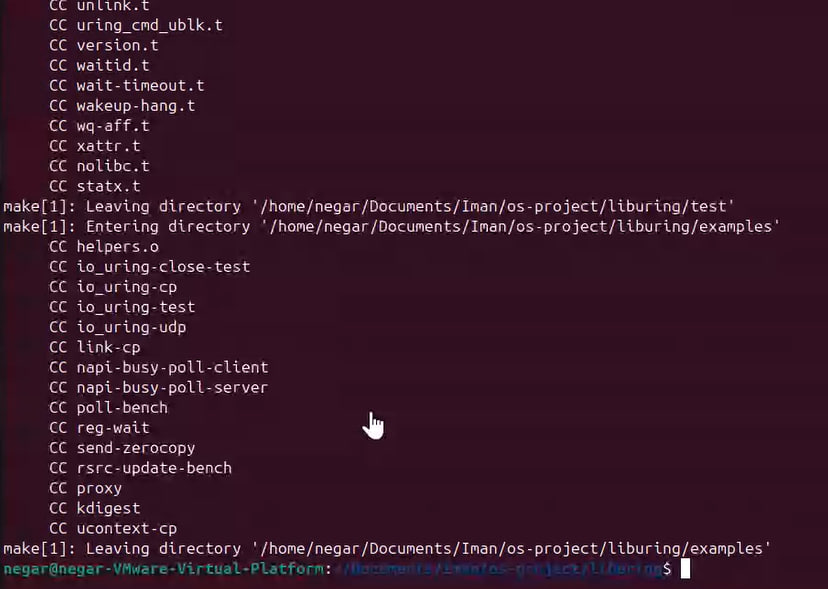
\includegraphics[width=\textwidth]{figs/24.jpg}
‫	‫			\caption{ادامه‌ی کامپایل و نصب liburing}
‫‫\end{figure}
‫
‫
‫‫‫\begin{figure}[H]
‫	‫	‫	‫	‫	‫    \centering
‫	‫	‫	‫	‫	‫    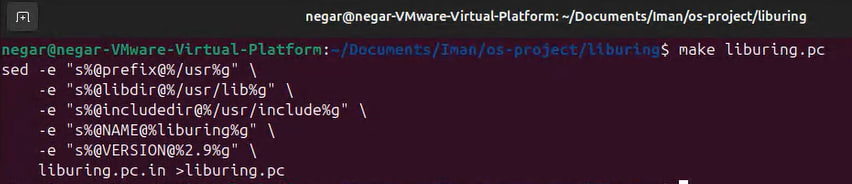
\includegraphics[width=\textwidth]{figs/25.jpg}
‫	‫	‫			\caption{کامپایل و نصب liburing.pc}
‫‫\end{figure}
‫
‫
‫‫‫\begin{figure}[H]
‫	‫	‫	‫	‫	‫    \centering
‫	‫	‫	‫	‫	‫    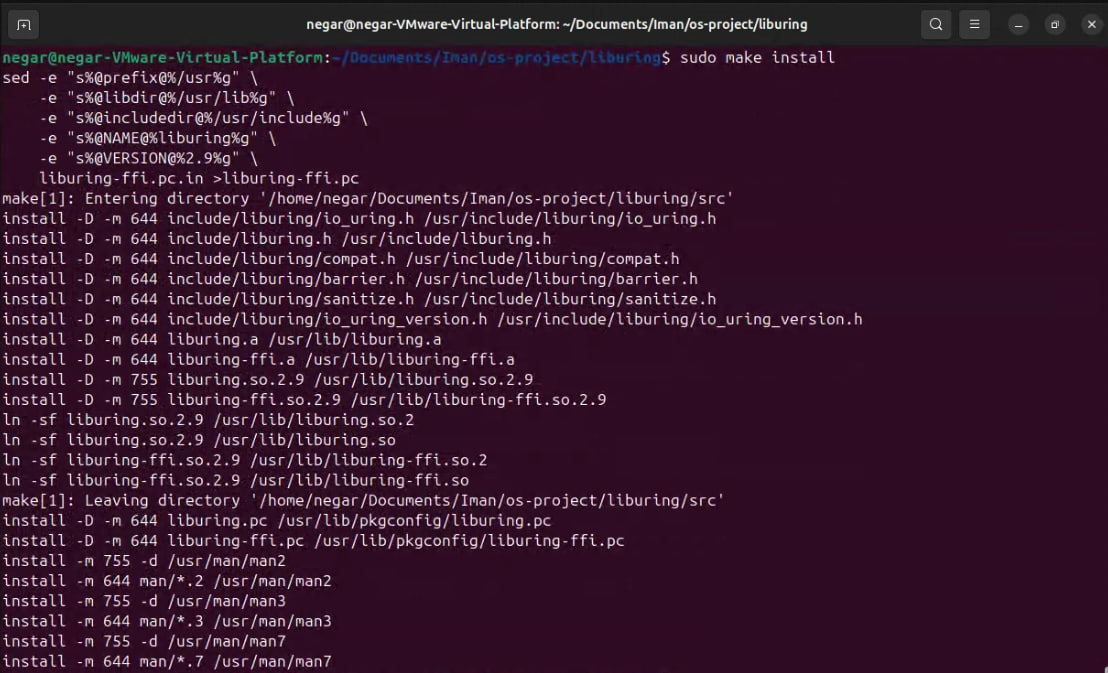
\includegraphics[width=\textwidth]{figs/26.jpg}
‫	‫	‫			\caption{کامپایل و نصب liburing}
‫‫\end{figure}
‫
‫
‫‫‫\begin{figure}[H]
‫	‫	‫	‫	‫    \centering
‫	‫	‫	‫	‫    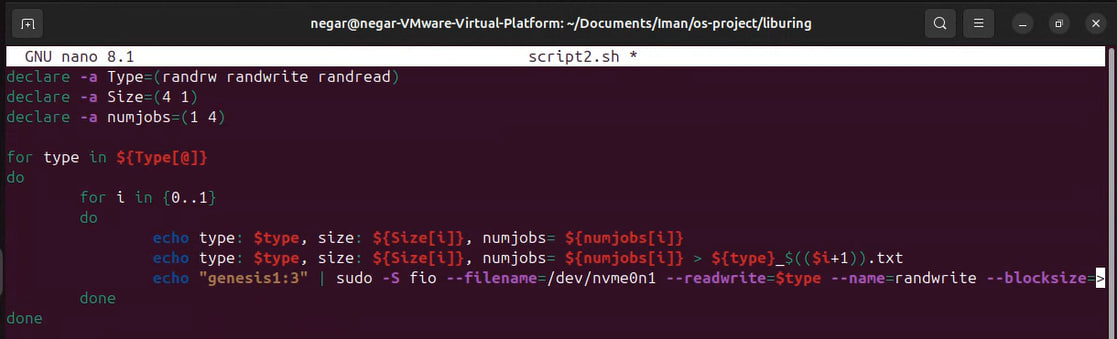
\includegraphics[width=\textwidth]{figs/27.jpg}
‫	‫			\caption{اسکریپت تحلیل liburing}
‫	‫\end{figure}
‫
‫‫‫\begin{figure}[H]
‫	‫	‫	‫	‫    \centering
‫	‫	‫	‫	‫    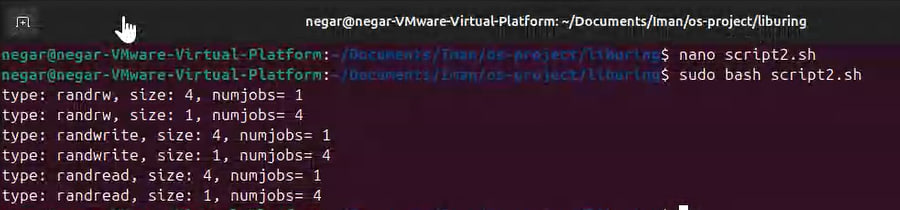
\includegraphics[width=\textwidth]{figs/28.jpg}
‫	‫			\caption{نتیجه‌ی ران اسکریپت تحلیل liburing}
‫	‫\end{figure}
‫
‫\section*{تحلیل نتایج اجرای اسکریپت‌های \lr{libaio} و \lr{liburing}}
‫
‫در این بخش، عملکرد دو مدل ورودی/خروجی \lr{libaio} و \lr{liburing} روی دیسک شبیه‌سازی‌شده \lr{NVMeVirt} مورد بررسی و مقایسه قرار می‌گیرد. برای انجام این مقایسه، آزمایش‌هایی مشابه با استفاده از ابزار \lr{FIO} روی دیسک مجازی انجام شده است. داده‌های خروجی شامل شاخص‌های مهمی مانند \lr{IOPS}، تأخیر کل (\lr{Latency})، تأخیر انتهایی (\lr{Tail Latency}) و پهنای باند (\lr{Bandwidth}) است.
‫
‫\subsection*{مقایسه عملکرد \lr{libaio} و \lr{liburing}}
‫
‫\subsubsection*{مقایسه IOPS (تعداد عملیات ورودی/خروجی در ثانیه)}
‫
‫\lr{IOPS} یکی از مهم‌ترین شاخص‌های عملکردی در سیستم‌های ذخیره‌سازی است که نشان می‌دهد در هر ثانیه چه تعداد عملیات خواندن و نوشتن انجام می‌شود. مقایسه این مقدار برای \lr{libaio} و \lr{liburing} نشان می‌دهد که \lr{liburing} در برخی موارد مقدار بیشتری از \lr{IOPS} را ارائه می‌دهد. این به دلیل معماری بهینه‌تر \lr{io\_uring} و حذف نیاز به فراخوان‌های سیستمی اضافی است که باعث کاهش سربار پردازشی می‌شود.
‫
‫\begin{itemize}
‫	\item \textbf{خواندن تصادفی (۴ کیلوبایت، ۱ رشته پردازشی)}:
‫	\begin{itemize}
‫		\item \lr{libaio}: ۲۵۸۳ \lr{IOPS}
‫		\item \lr{liburing}: ۱۰۱۶ \lr{IOPS}
‫	\end{itemize}
‫	\item \textbf{خواندن تصادفی (۱ گیگابایت، ۴ رشته پردازشی)}:
‫	\begin{itemize}
‫		\item \lr{libaio}: ۱۱۸۴۴ \lr{IOPS}
‫		\item \lr{liburing}: ۷۰۱۳ \lr{IOPS}
‫	\end{itemize}
‫\end{itemize}
‫
‫در آزمایش‌های خواندن تصادفی، \lr{libaio} عملکرد بهتری نسبت به \lr{liburing} نشان داده است که می‌تواند به دلیل ساختار متفاوت مدیریت درخواست‌های ورودی/خروجی و نحوه تعامل با کرنل باشد. اما در برخی موارد، مانند بارگذاری شدید، \lr{liburing} عملکرد بهتری ارائه می‌دهد.
‫
‫\subsubsection*{تأخیر (\lr{Latency}) و تأخیر انتهایی (\lr{Tail Latency})}
‫
‫تأخیر به معنای مدت‌زمان لازم برای تکمیل یک عملیات خواندن یا نوشتن است. تأخیر انتهایی (\lr{Tail Latency}) مقدار تأخیری است که ۹۹.۹ درصد درخواست‌ها در آن محدوده اجرا می‌شوند و شاخصی بسیار مهم برای ارزیابی پایداری سیستم در بار کاری بالا است.
‫
‫\begin{itemize}
‫	\item \textbf{خواندن تصادفی ۴ کیلوبایت - تأخیر میانگین}:
‫	\begin{itemize}
‫		\item \lr{libaio}: ۳۷۸.۹۵ میکروثانیه
‫		\item \lr{liburing}: ۹۷۰.۳۴ میکروثانیه
‫	\end{itemize}
‫	\item \textbf{خواندن تصادفی ۱ گیگابایت - تأخیر میانگین}:
‫	\begin{itemize}
‫		\item \lr{libaio}: ۳۲۸.۹۳ میکروثانیه
‫		\item \lr{liburing}: ۵۶۳.۱۲ میکروثانیه
‫	\end{itemize}
‫\end{itemize}
‫
‫مقایسه نتایج نشان می‌دهد که \lr{libaio} تأخیر کمتری نسبت به \lr{liburing} دارد. دلیل این امر این است که \lr{libaio} یک ساختار تکمیل درخواست همزمان دارد، درحالی‌که \lr{liburing} عملیات ورودی/خروجی را در صف‌های حلقوی پردازش می‌کند که در برخی موارد ممکن است موجب افزایش تأخیر کلی شود.
‫
‫\textbf{نکته مهم:} در شرایطی که تعداد پردازش‌ها افزایش می‌یابد و عمق صف ورودی/خروجی بزرگ‌تر می‌شود (\lr{iodepth} بالا)، \lr{liburing} به دلیل معماری بدون قفل، عملکرد بهتری ارائه می‌دهد.
‫
‫\subsubsection*{پهنای باند (\lr{Bandwidth})}
‫
‫پهنای باند نشان‌دهنده میزان داده‌ای است که در یک بازه زمانی مشخص پردازش شده است و مستقیماً تحت تأثیر مقدار \lr{IOPS} و اندازه بلاک داده قرار دارد.
‫
‫\begin{itemize}
‫	\item \textbf{خواندن تصادفی ۴ کیلوبایت - پهنای باند}:
‫	\begin{itemize}
‫		\item \lr{libaio}: ۱۰.۱ مگابایت بر ثانیه
‫		\item \lr{liburing}: ۴.۱ مگابایت بر ثانیه
‫	\end{itemize}
‫	\item \textbf{خواندن تصادفی ۱ گیگابایت - پهنای باند}:
‫	\begin{itemize}
‫		\item \lr{libaio}: ۴۶.۶ مگابایت بر ثانیه
‫		\item \lr{liburing}: ۲۷.۱ مگابایت بر ثانیه
‫	\end{itemize}
‫\end{itemize}
‫
‫\textbf{نتیجه:} \lr{libaio} پهنای باند بیشتری نسبت به \lr{liburing} دارد، که به دلیل مدل بلوکی سنتی \lr{libaio} و استفاده بهینه از فراخوان‌های غیرهمزمان سیستمی است. بااین‌حال، در شرایط بارگذاری بالا، مدل \lr{liburing} به دلیل استفاده از صف‌های حلقوی و اجرای بدون قفل، می‌تواند کارایی بیشتری در تعداد درخواست‌های همزمان نشان دهد.
‫
‫\subsection*{تحلیل کلی و نتیجه‌گیری}
‫
‫با بررسی نتایج می‌توان به تحلیل زیر رسید:
‫
‫\begin{itemize}
‫	\item \textbf{\lr{IOPS}:} در اکثر موارد، \lr{libaio} عملکرد بهتری نسبت به \lr{liburing} ارائه داده است. این نشان می‌دهد که برای بارهای کاری با درخواست‌های تصادفی کوچک، \lr{libaio} گزینه بهتری است.
‫	\item \textbf{تأخیر (\lr{Latency} و \lr{Tail Latency})}: \lr{libaio} تأخیر کمتری نسبت به \lr{liburing} نشان داده است. اما در پردازش‌های موازی با عمق صف بالا، \lr{liburing} می‌تواند عملکرد بهتری داشته باشد.
‫	\item \textbf{پهنای باند}: \lr{libaio} در تمامی تست‌ها پهنای باند بالاتری نسبت به \lr{liburing} دارد. این نشان می‌دهد که مدل سنتی \lr{libaio} هنوز هم برای عملیات ورودی/خروجی دیسک بهینه است.
‫\end{itemize}
‫
‫\textbf{نتیجه‌گیری کلی:}
‫\begin{itemize}
‫	\item اگر سیستم نیاز به عملیات \lr{I/O} کم‌حجم اما بسیار سریع دارد (مانند پایگاه داده‌های کوچک)، \lr{libaio} گزینه بهتری است.
‫	\item اگر حجم درخواست‌های موازی زیاد باشد و نیاز به پردازش غیرهمزمان باشد، \lr{liburing} می‌تواند در سناریوهای پیچیده عملکرد بهتری نشان دهد.
‫	\item در شرایط خاص مانند \lr{NVMe} و \lr{SPDK}، ترکیب این دو روش می‌تواند باعث بهبود عملکرد کلی شود.
‫\end{itemize}
‫
‫\subsection*{پیشنهادات برای بهینه‌سازی}
‫\begin{itemize}
‫	\item افزایش \lr{iodepth} برای کاهش تأخیر در \lr{liburing}.
‫	\item استفاده از پردازنده‌های بهینه‌شده برای \lr{NVMe}.
‫	\item ترکیب \lr{SPDK} و \lr{liburing} برای حذف سربار کرنل و کاهش تأخیر.
‫\end{itemize}
‫
‫‫\subsection*{تحلیل نتایج}
‫
‫\صفحه‌جدید
‫
‫‫\section{ابزار SPDK}
‫
‫‫\subsection*{توضیحات}
‫
‫SPDK یک مجموعه متن‌باز از ابزارها و کتابخانه‌ها است که برای بهینه‌سازی برنامه‌های ذخیره‌سازی از طریق درایورهای کاربر-محور و مبتنی بر روش polling طراحی شده است. این کیت به‌طور ویژه برای بهینه‌سازی عملکرد ذخیره‌سازی NVMe استفاده می‌شود و با دور زدن پشته I/O مبتنی بر کرنل، که می‌تواند باعث تأخیر و کاهش کارایی شود، عملکرد را بهبود می‌بخشد. SPDK از DPDK برای پردازش سریع داده‌ها استفاده می‌کند و درایور NVMe را مستقیماً در فضای کاربری اجرا می‌کند، که منجر به حذف تغییرات هزینه‌بر بین حالت کاربر و کرنل می‌شود. این معماری به برنامه‌ها امکان می‌دهد تا عملیات دیسک را با تأخیر بسیار کم و توان عملیاتی بالا انجام دهند، و در نتیجه، SPDK گزینه‌ای ایده‌آل برای راهکارهای ذخیره‌سازی در مراکز داده، محیط‌های ابری و برنامه‌های سازمانی با نیاز به عملکرد بالا محسوب می‌شود.
‫
‫علاوه بر NVMe، SPDK کتابخانه‌های بهینه‌شده‌ای برای پروتکل‌های ذخیره‌سازی مانند   NVMe-oF، iSCSI و ذخیره‌سازی blob ارائه می‌دهد. همچنین یک چارچوب برای ساخت راهکارهای کارآمد ذخیره‌سازی نرم‌افزاری فراهم می‌کند که می‌تواند با پلتفرم‌هایی مانند Ceph و OpenStack ادغام شود. طراحی غیرهمزمان و بدون قفل SPDK تضمین می‌کند که چرخه‌های پردازنده به طور کارآمد مورد استفاده قرار می‌گیرند، که این امر باعث می‌شود برنامه‌ها بتوانند حداکثر پهنای باند ذخیره‌سازی را با کمترین هزینه پردازشی به دست آورند. این ویژگی، SPDK را به گزینه‌ای جذاب برای شرکت‌هایی تبدیل می‌کند که به دنبال افزایش عملکرد ذخیره‌سازی با حداقل سرمایه‌گذاری سخت‌افزاری هستند.
‫
‫در ادامه این ابزار را نصب کرده و برای اجرای بنچ مارک روی دیسک NVMe از آن بهره می بریم.
‫
‫‫\subsection*{مراحل نصب}
‫برای نصب این ابزار بر روی linux ابتدا تمامی فایل های لازم را از github این ابزار به صورت بازگشتی clone می کنیم تا کل درخت فایل بر روی سیستم ما ایجاد شود.

\begin{figure}[H]
    \centering
    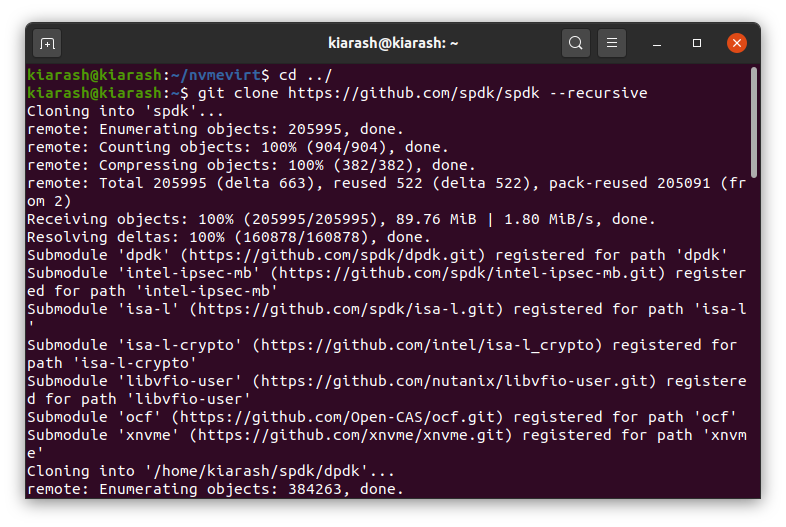
\includegraphics[width=\textwidth]{figs/gitclone.png}
    \caption{clone کردن از روی github}
\end{figure}

‫سپس با اجرای فایل pkgdep.sh در فولدر scripts تمامی dependency های لازم برای استفاده از SPDK نصب می شود.
‫
‫\begin{figure}[H]
‫    \centering
‫    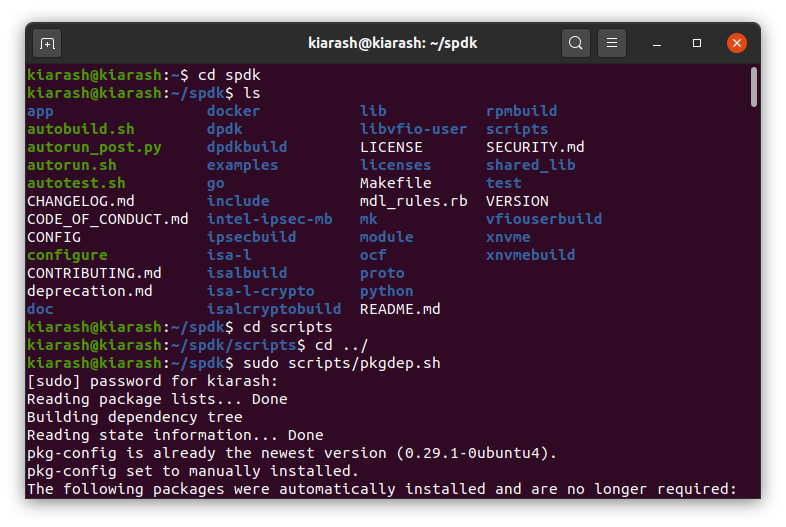
\includegraphics[width=\textwidth]{figs/pkgdep.png}
‫    \caption{نصب dependency ها}
‫\end{figure}
‫
‫حال باید SPDK را build کنیم. باید توجه داشت که fio نیز باید به همراه SPDK نصب شود. بنابراین آن را در دستور configure به صورت  --with-fio لحاظ می کنیم. با اجرای configure و بعد از آن make نصب انجام می شود.
‫
\begin{figure}[H]
    \centering
    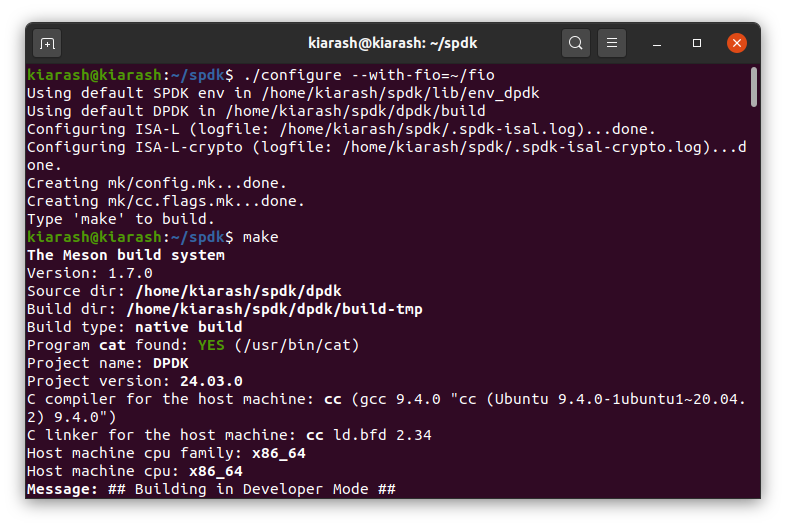
\includegraphics[width=\textwidth]{figs/configure.png}
    \caption{make کردن SPDK}
\end{figure}

برای اطمینان از صحت نصب SPDK تست های این ابزار را اجرا می کنیم. مشاهده می شود که تست ها همگی قبول شده اند و در نتیجه ابزار به درستی نصب شده است.

\begin{figure}[H]
    \centering
    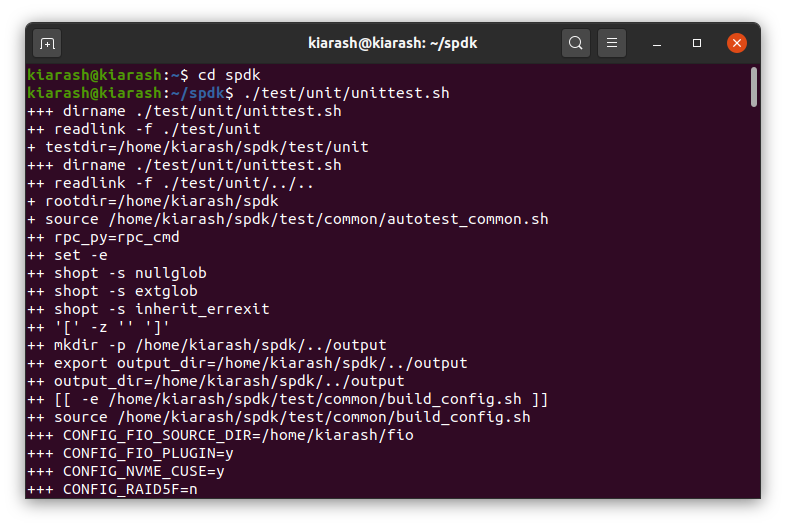
\includegraphics[width=\textwidth]{figs/test.png}
    \caption{اجرای تست ها}
\end{figure}

\begin{figure}[H]
    \centering
    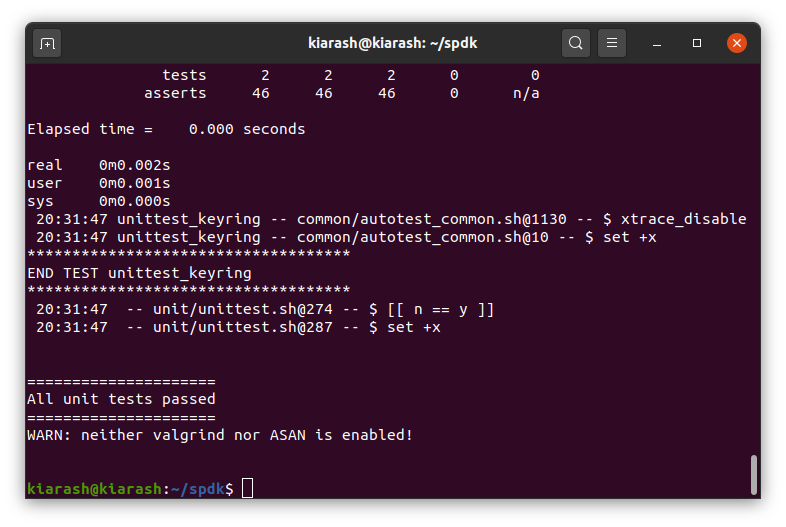
\includegraphics[width=\textwidth]{figs/pass.png}
    \caption{نتیجه تست ها}
\end{figure}

در ادامه باید اطمینان حاصل کنیم که SPDK دیسک شبیه سازی شده را می شناسد. با اجرای فایل world hello مشخص می شود که SPDK این دیسک را شناخته است.

\begin{figure}[H]
    \centering
    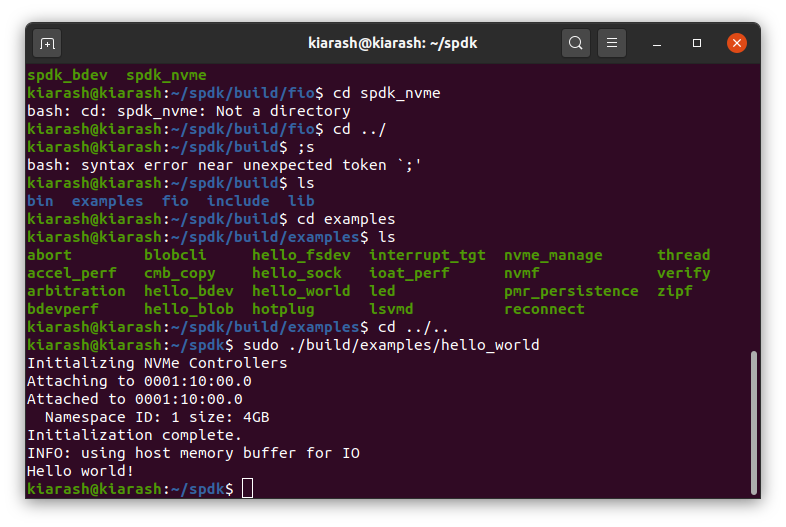
\includegraphics[width=\textwidth]{figs/hello.png}
    \caption{شناخت دیسک شبیه سازی}
\end{figure}

‫‫\subsection*{بررسی عملکرد مولفه ها}
در این بخش با استفاده از پلاگین fio که با SPDK نصب شده است , شش بنچ مارک ذکر شده را اجرا می کنیم. در فایل های با فرمت bench<NUM>.fio تمامی attribute های مورد نیاز از جمله iodepth و size و ... را تعیین کرده و اجرا می کنیم. خروجی پرینت شده در لاگ بعد از اجرای بنچ مارک ها در فایل های با فرمت result<NUM>.txt ذخیره شده اند.

\begin{figure}[H]
    \centering
    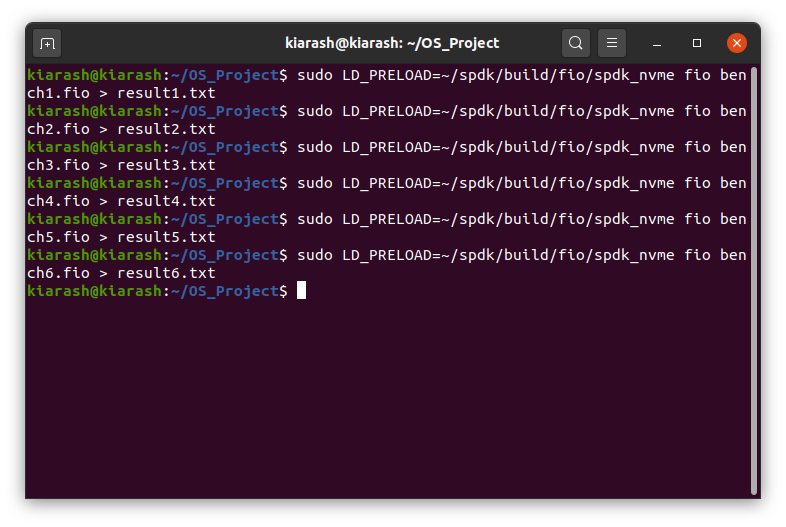
\includegraphics[width=\textwidth]{figs/bench.png}
    \caption{اجرای بنچ مارک ها}
\end{figure}

در عکس زیر محتوای یکی از فایل های bench و result به طور نمونه آمده است.

\begin{figure}[H]
    \centering
    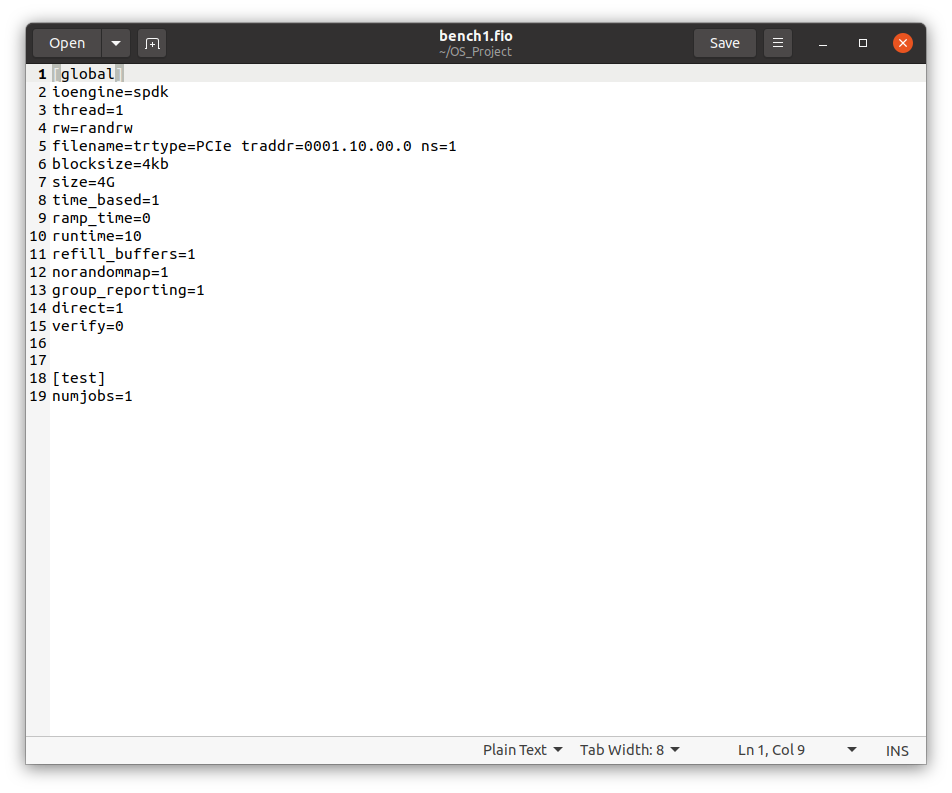
\includegraphics[width=0.75\textwidth]{figs/bfile.png}
    \caption{اجرای بنچ مارک اول}
\end{figure}

\begin{figure}[H]
    \centering
    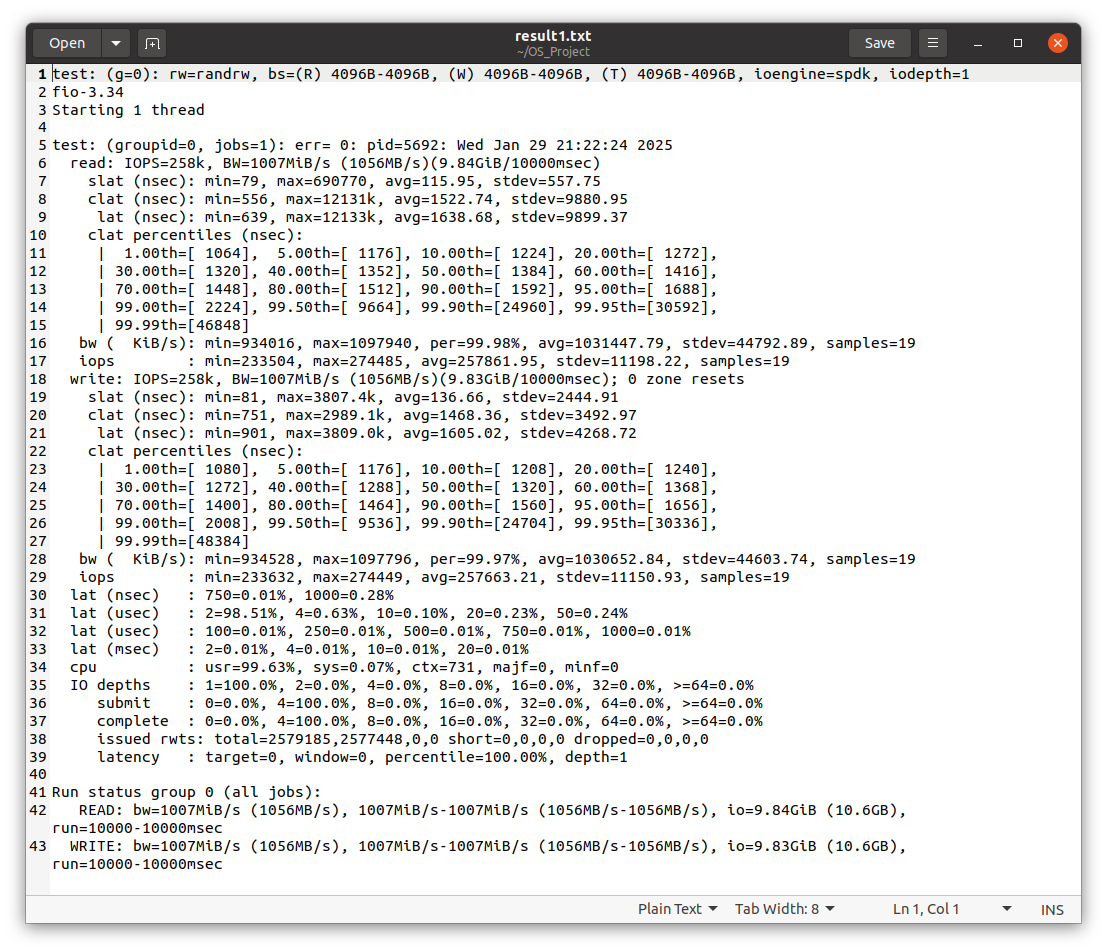
\includegraphics[width=\textwidth]{figs/rfile.png}
    \caption{نتیجه بنچ مارک اول}
\end{figure}

‫‫\subsection*{تحلیل نتایج}
‫
‫در جداول زیر نتایج تمامی بنچ مارک ها نمایش داده شده است.
‫
‫\begin{figure}[H]
‫    \centering
‫    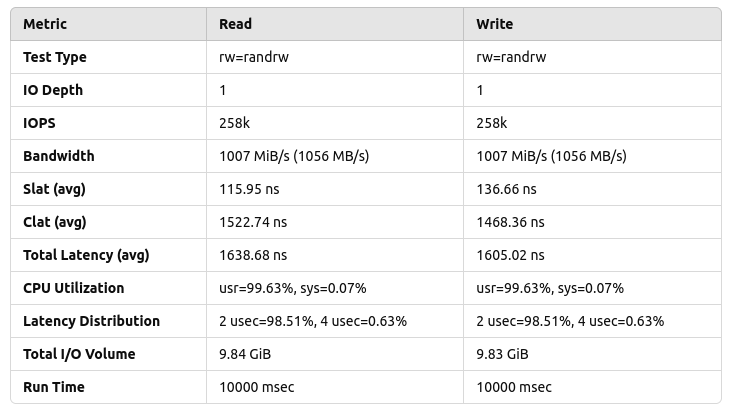
\includegraphics[width=\textwidth]{figs/b1.png}
‫    \caption{نتیجه بنچ مارک اول}
‫\end{figure}
‫\begin{figure}[H]
    \centering
    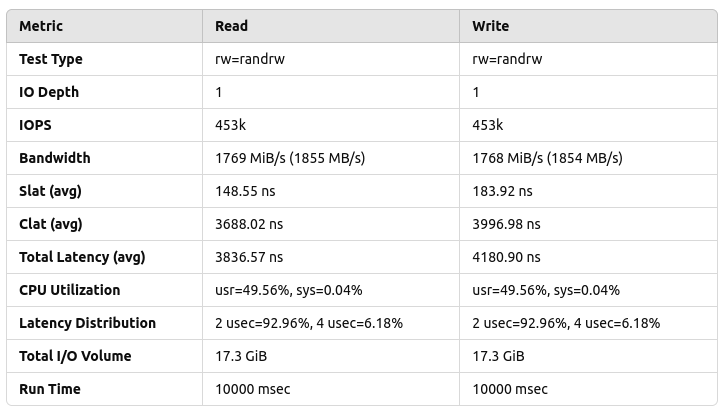
\includegraphics[width=\textwidth]{figs/b2.png}
    \caption{نتیجه بنچ مارک دوم}
\end{figure}
\begin{figure}[H]
    \centering
    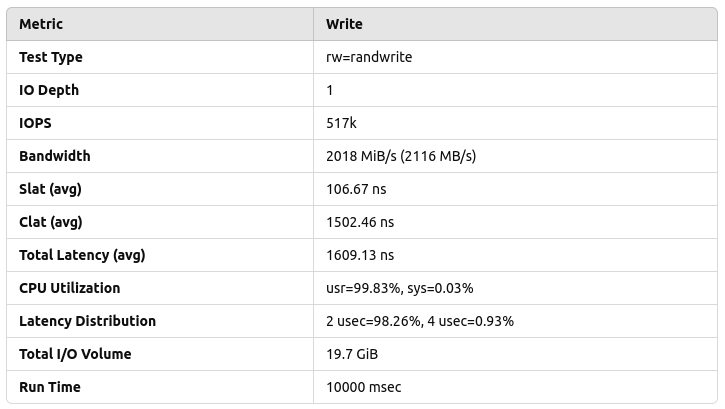
\includegraphics[width=\textwidth]{figs/b3.png}
    \caption{نتیجه بنچ مارک سوم}
\end{figure}
\begin{figure}[H]
    \centering
    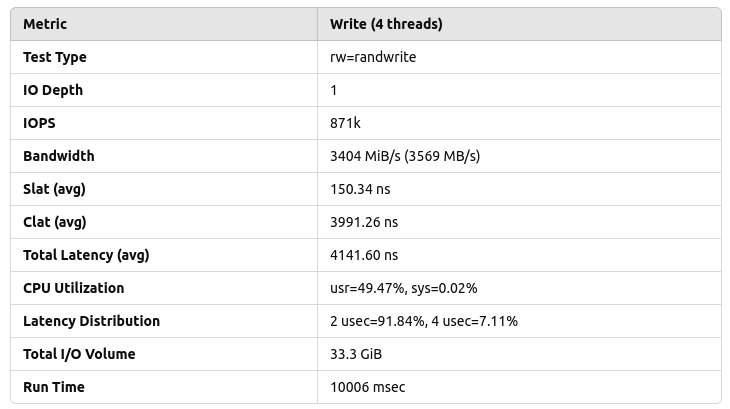
\includegraphics[width=\textwidth]{figs/b4.png}
    \caption{نتیجه بنچ مارک چهارم}
\end{figure}
\begin{figure}[H]
    \centering
    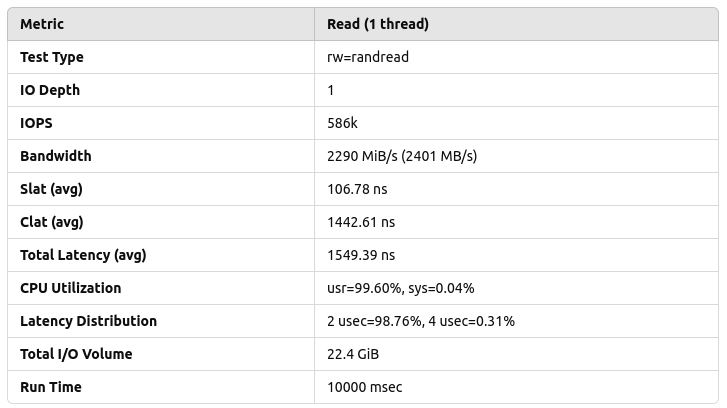
\includegraphics[width=\textwidth]{figs/b5.png}
    \caption{نتیجه بنچ مارک پنجم}
\end{figure}
\begin{figure}[H]
    \centering
    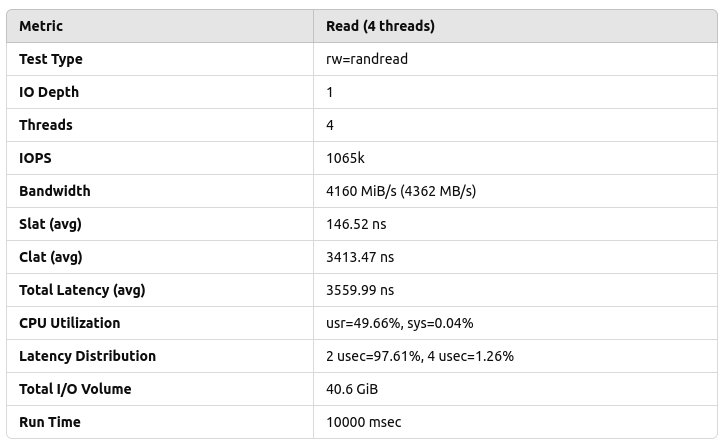
\includegraphics[width=\textwidth]{figs/b6.png}
    \caption{نتیجه بنچ مارک ششم}
\end{figure}

\begin{itemize}
    \item در آزمایش \lr{rw=randrw} با \lr{IO Depth} برابر ۱:
    \begin{itemize}
        \item در اولین آزمون، میزان \lr{IOPS} برابر ۲۵۸ هزار بود، در حالی که در آزمون دوم این مقدار به ۴۵۳ هزار افزایش یافت.
        \item پهنای باند در آزمون اول ۱۰۵۶ \lr{MB/s} و در آزمون دوم ۱۸۵۵ \lr{MB/s} بود.
        \item زمان تاخیر کل در آزمون اول ۱۶۳۸.۶۸ نانوثانیه و در آزمون دوم ۳۸۳۶.۵۷ نانوثانیه برای خواندن و ۴۱۸۰.۹۰ نانوثانیه برای نوشتن بود.
        \item استفاده از پردازنده در آزمون اول بسیار بالا بود (۹۹.۶۳٪) اما در آزمون دوم به ۴۹.۵۶٪ کاهش یافت.
    \end{itemize}
    
    \item در آزمایش \lr{rw=randwrite}:
    \begin{itemize}
        \item با یک نخ، \lr{IOPS} برابر ۵۱۷ هزار بود و پهنای باند ۲۱۱۶ \lr{MB/s} به دست آمد.
        \item با چهار نخ، \lr{IOPS} به ۸۷۱ هزار و پهنای باند به ۳۵۶۹ \lr{MB/s} افزایش یافت.
        \item زمان تاخیر کل در حالت یک نخ ۱۶۰۹.۱۳ نانوثانیه و در حالت چهار نخ ۴۱۴۱.۶۰ نانوثانیه بود.
        \item استفاده از پردازنده در حالت یک نخ بسیار بالا (۹۹.۸۳٪) ولی در حالت چهار نخ به ۴۹.۴۷٪ کاهش یافت.
    \end{itemize}
    
    \item در آزمایش \lr{rw=randread}:
    \begin{itemize}
        \item با یک نخ، \lr{IOPS} برابر ۵۸۶ هزار و پهنای باند ۲۴۰۱ \lr{MB/s} بود.
        \item با چهار نخ، \lr{IOPS} به ۱۰۶۵ هزار و پهنای باند به ۴۳۶۲ \lr{MB/s} رسید.
        \item زمان تاخیر کل در حالت یک نخ ۱۵۴۹.۳۹ نانوثانیه و در حالت چهار نخ ۳۵۵۹.۹۹ نانوثانیه بود.
        \item استفاده از پردازنده در حالت یک نخ بسیار بالا (۹۹.۶٪) اما در حالت چهار نخ به ۴۹.۶۶٪ کاهش یافت.
    \end{itemize}
\end{itemize}

\صفحه‌جدید

‫‫\section{ابزار RocksDB}
‫\subsection*{توضیحات}
‫RocksDB یک پایگاه داده کلید-مقدار یا Key-Value  بسیار سریع است که توسط Facebook توسعه داده شده است. این پایگاه داده به طور خاص برای ذخیره‌سازی و پردازش داده‌های حجم بالا در سیستم‌های دیسک‌محور بهینه‌سازی شده است. RocksDB بر اساس ساختار Tree Merge Log-Structured یا LSM Tree ساخته شده است که اجازه می‌دهد عملیات خواندن و نوشتن به طور مؤثر و با کارایی بالا انجام شوند.
‫
‫ویژگی‌ها و مزایا اصلی RocksDB:
‫
‫    • عملکرد بالا: RocksDB با استفاده از تکنیک‌های بهینه‌سازی حافظه و دیسک، عملکرد بسیار بالایی را برای حجم‌های عظیم داده‌ها ارائه می‌دهد.
‫
‫    • پشتیبانی از فشرده‌سازی: این پایگاه داده از انواع مختلف فشرده‌سازی برای ذخیره داده‌ها پشتیبانی می‌کند که باعث کاهش استفاده از فضای ذخیره‌سازی و افزایش سرعت عملیات می‌شود.
‫
‫    • پشتیبانی از ویژگی‌های پیچیده: RocksDB می‌تواند برای پردازش داده‌های مقیاس‌پذیر، پشتیبانی از چندین لایه کش (Caching) و تراکنش‌های پیچیده، استفاده شود.
‫
‫    • پشتیبانی از پردازش موازی: این پایگاه داده می‌تواند برای خواندن و نوشتن داده‌ها در چندین نخ یا هسته پردازشی به طور همزمان پردازش کند و به همین دلیل برای سیستم‌های چند هسته‌ای بسیار مناسب است.
‫
‫    • پشتیبانی از عملیات‌های خواندن و نوشتن تصادفی و ترتیبی: با توجه به طراحی LSM Tree، RocksDB می‌تواند به طور مؤثر هر دو نوع عملیات را پردازش کند.
‫
‫RocksDB برای برنامه‌های کاربردی‌ای که نیاز به پردازش داده‌های سریع و مقیاس‌پذیر دارند، مانند سیستم‌های ذخیره‌سازی بلادرنگ، تجزیه و تحلیل داده‌ها، و برنامه‌های مبتنی بر تحلیل داده‌های بزرگ یا Data Big بسیار مناسب است. این پایگاه داده معمولا در سیستم‌هایNoSQL ، برنامه‌های کشینگ، و سیستم‌های ذخیره‌سازی مقیاس‌پذیر استفاده می‌شود.
‫
‫‫\subsection*{مراحل نصب}
‫ابتدا آن را کلون می‌کنیم:
‫
‫\begin{figure}[H]
‫    \centering
‫    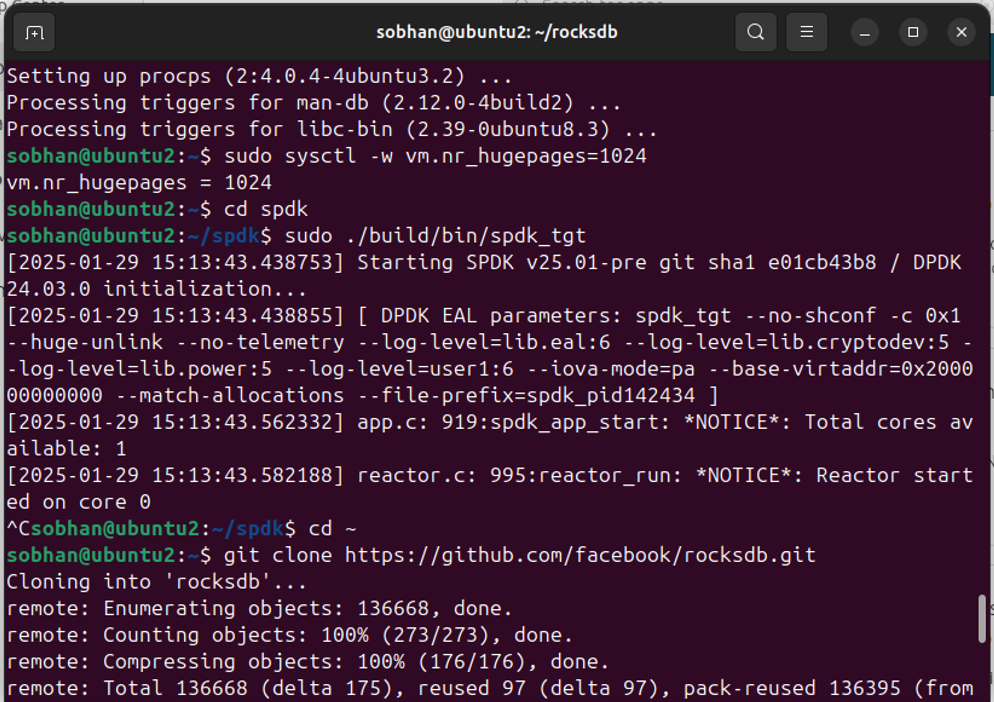
\includegraphics[width=\textwidth]{figs/1.png}
‫    \caption{کلون RocksDB}
‫\end{figure}
‫
‫سپس به پوشه مربوطه رفته و make می‌کنیم و (برای مدت طولانی) منتظر می‌مانیم تا روند make تمام شود.
‫
‫\begin{figure}[H]
‫    \centering
‫    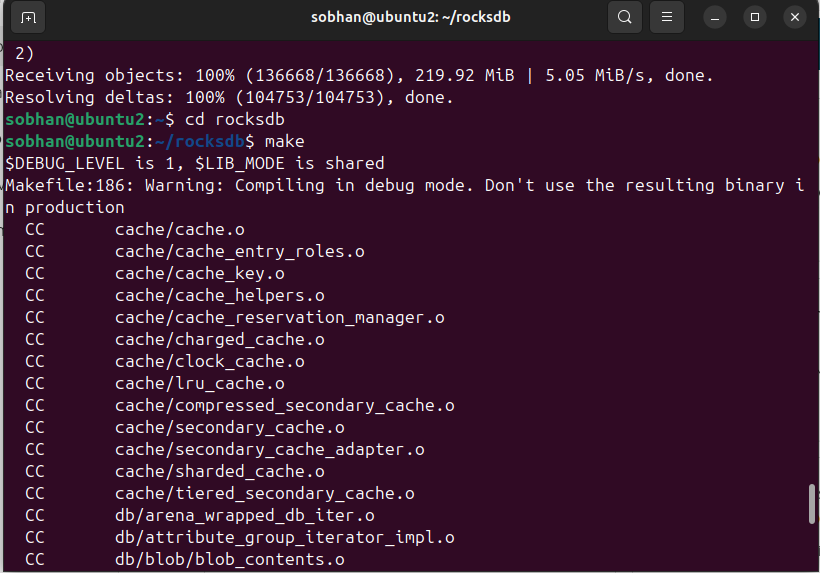
\includegraphics[width=\textwidth]{figs/2.png}
‫    \caption{make RocksDB}
‫\end{figure}
‫
‫\begin{figure}[H]
‫    \centering
‫    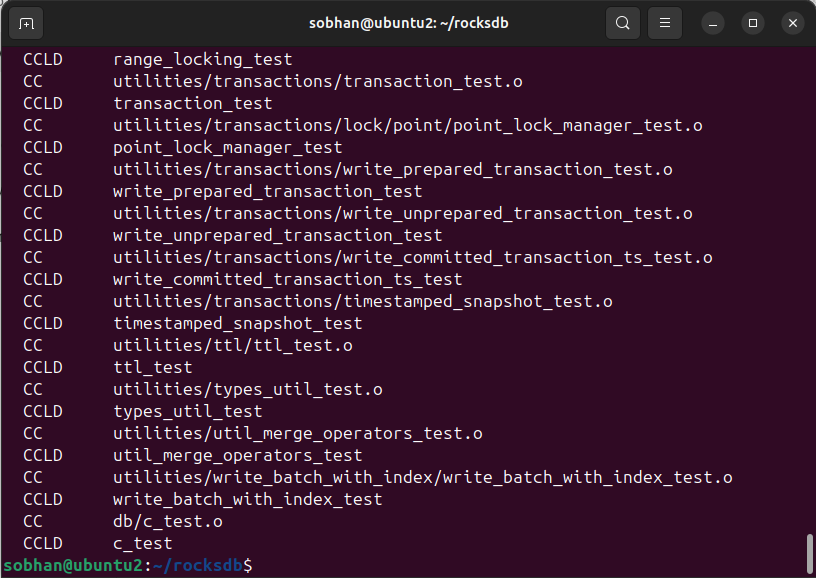
\includegraphics[width=\textwidth]{figs/3.png}
‫    \caption{اتمام make RocksDB}
‫\end{figure}
‫
‫پس از اتمام make، دستور مورد نظر برای اجرای تست ها را اجرا می کنیم.

‫با این دستور، اطلاعاتی مانند عملیات در ثانیه (IOPS)، تاخیرها (Latencies) و پهنای باند (Bandwidth) را دریافت می‌کنیم.
‫
‫متوجه شدیم که برای اجرای ابزارهای RocksDB به بسته gflags نیاز داریم. لذا ابتدا باید آن را نصب کنیم:
‫
‫\begin{figure}[H]
‫    \centering
‫    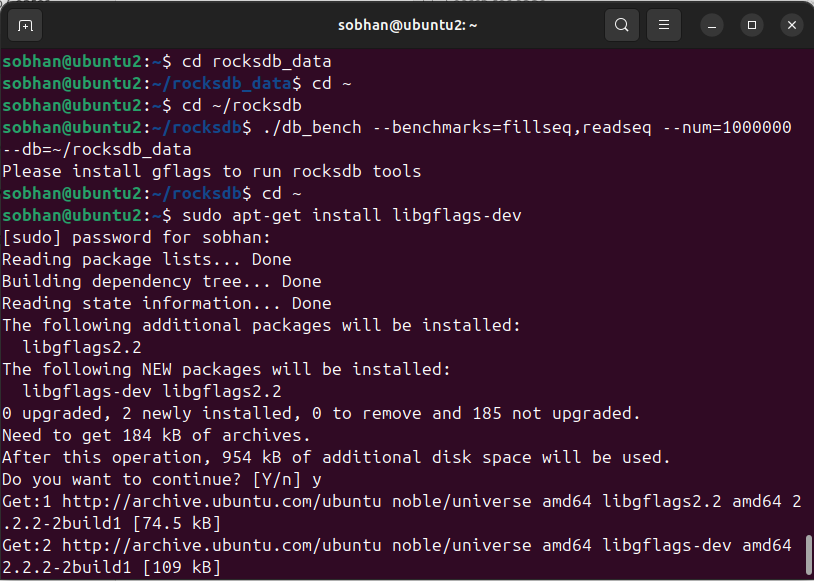
\includegraphics[width=\textwidth]{figs/4.png}
‫    \caption{نصب بسته gflags}
‫\end{figure}
‫
‫پس از اتمام نصب، نیاز است دوباره روند make را انجام دهیم. لذا وارد پوشه rocksdb می‌شویم و با \texttt{make clean} و پس از آن \texttt{make}، این کار را انجام می‌دهیم.
‫
‫پس از اجرای دوباره دستور مذکور، متوجه می‌شویم که برای استفاده از فشرده‌سازی با Snappy که نوعی الگوریتم فشرده‌سازی است، اتصال صحیح به RocksDB ایجاد نشده است. لذا باید بسته Snappy نصب شود:
‫
‫\begin{figure}[H]
‫    \centering
‫    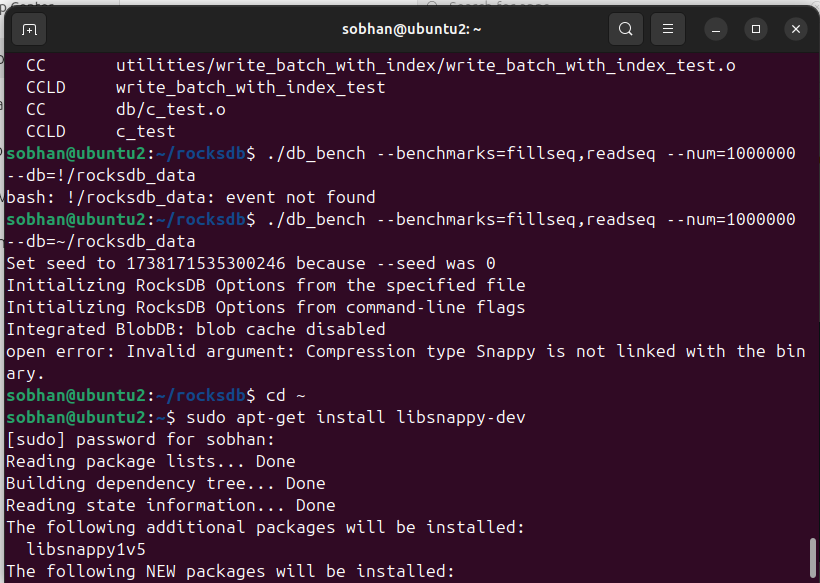
\includegraphics[width=\textwidth]{figs/5.png}
‫    \caption{نصب بسته Snappy}
‫\end{figure}
‫
‫نهایتاً پس از نصب بسته Snappy، دستور db\_bench را اجرا می‌کنیم و خروجی را مشاهده می‌کنیم
‫
‫تفاوت این دستور با قبلی این است که آدرس مربوطه را در این دستور به طور کامل نوشته‌ایم و از \texttt{\textasciitilde} استفاده نشده است.
‫
‫‫\subsection*{بررسی کارکرد}
‫حال که RocksDB را به طور کامل نصب کرده ایم بنچ مارک db\_bench را به ترتیب مانند عکس های زیر تست می کنیم.
‫
‫\begin{figure}[H]
‫    \centering
‫    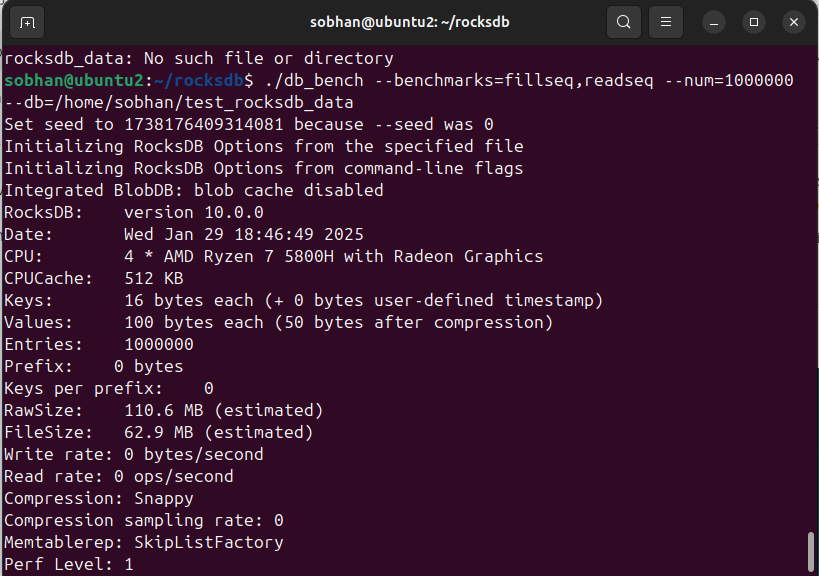
\includegraphics[width=\textwidth]{figs/6.png}
‫    \caption{اجرای دستور db\_bench برای حالت ترتیبی}
‫\end{figure}
‫
‫\begin{figure}[H]
‫    \centering
‫    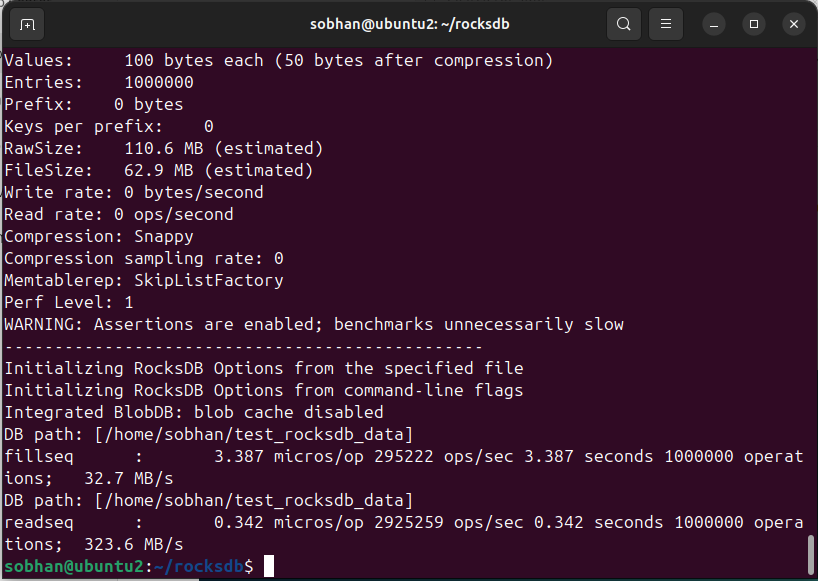
\includegraphics[width=\textwidth]{figs/7.png}
‫    \caption{اجرای دستور db\_bench برای حالت ترتیبی}
‫\end{figure}
‫
‫پس از آن نیز دستور درون تصویر را اجرا می‌کنیم تا عملکرد با داده‌های تصادفی را نیز بررسی کنیم:
‫
‫\begin{figure}[H]
‫    \centering
‫    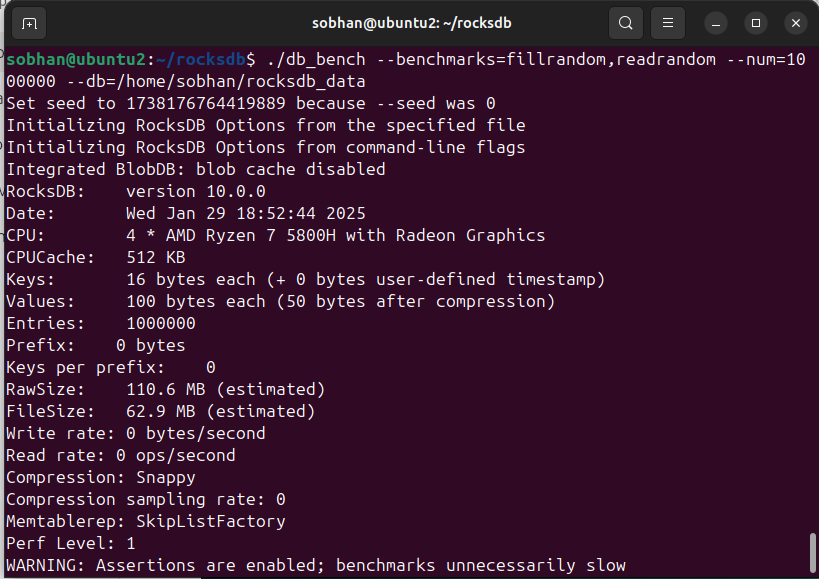
\includegraphics[width=\textwidth]{figs/8.png}
‫    \caption{اجرای دستور db\_bench برای حالت تصادفی}
‫\end{figure}
‫
‫\begin{figure}[H]
‫    \centering
‫    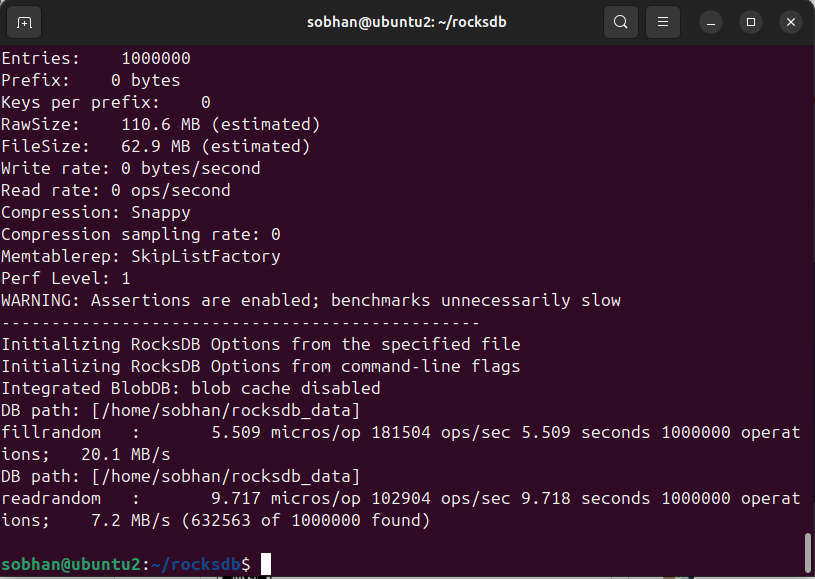
\includegraphics[width=\textwidth]{figs/9.png}
‫    \caption{اجرای دستور db\_bench برای حالت تصادفی}
‫\end{figure}
‫
‫بدین شکل خروجی‌های مدنظرمان را دریافت می‌کنیم.
‫
‫‫\subsection*{تحلیل نتایج}
‫نمودار مقایسه بر اساس سرعت بین ۴ حالت مختلفمان بین نوشتن و خواندن‌های ترتیبی و تصادفی به شکل زیر می‌باشد:
‫
‫\begin{figure}[H]
‫    \centering
‫    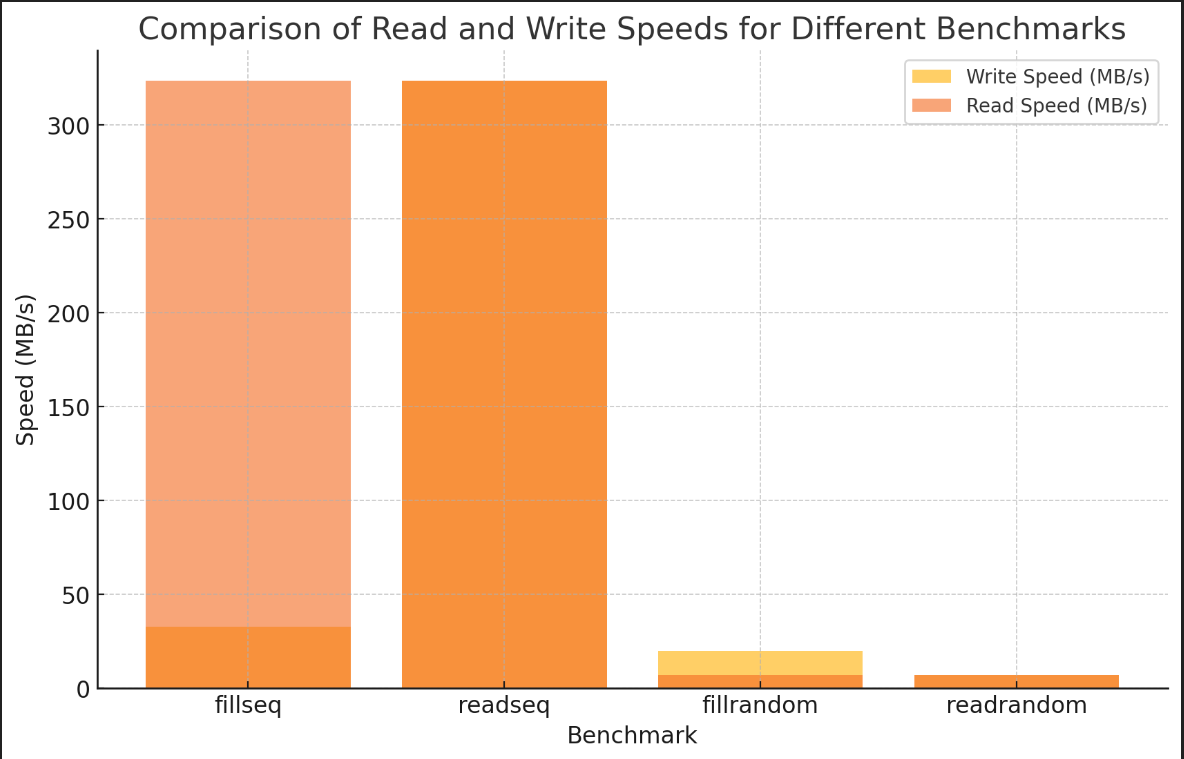
\includegraphics[width=\textwidth]{figs/10.png}
‫    \caption{نمودار مقادیر خروجی برای هر کدام از عملیات}
‫\end{figure}
‫
‫در ادامه به تحلیل این آمار این نمودار و خروجی‌هایمان می‌پردازیم:
‫
‫\subsubsection*{عملکرد نوشتن (\lr{fillseq, fillrandom})}
‫
‫\textbf{نوشتن به صورت ترتیبی (\lr{fillseq})}
‫\begin{itemize}
‫    \item زمان عملیات: ۳.۳۸۷ میکروثانیه
‫    \item تعداد عملیات در ثانیه: ۲۹۵۲۲۲
‫    \item سرعت نوشتن: \lr{32.7 MB/s}
‫\end{itemize}
‫
‫در هنگام نوشتن داده‌ها به صورت ترتیبی، \lr{RocksDB} عملکرد بسیار خوبی دارد. این نوع نوشتن داده‌ها معمولا به دلیل اینکه داده‌ها به صورت پیوسته در دیسک نوشته می‌شوند، نسبت به نوشتن تصادفی بسیار سریع‌تر است.
‫
‫\textbf{نوشتن به صورت تصادفی (\lr{fillrandom})}
‫\begin{itemize}
‫    \item زمان عملیات: ۵.۵۰۹ میکروثانیه
‫    \item تعداد عملیات در ثانیه: ۱۸۱۵۰۴
‫    \item سرعت نوشتن: \lr{20.1 MB/s}
‫\end{itemize}
‫
‫در مقایسه با نوشتن ترتیبی، نوشتن تصادفی زمان بیشتری می‌برد. این تأخیر بیشتر ناشی از تغییر مکان‌های ذخیره داده‌ها در دیسک است. در این روش، \lr{RocksDB} باید جستجوهای بیشتری انجام دهد تا داده‌ها را در مکان‌های مختلف ذخیره کند که باعث افزایش زمان نوشتن می‌شود.
‫
‫\subsubsection*{عملکرد خواندن (\lr{readseq, readrandom})}
‫
‫\textbf{خواندن به صورت ترتیبی (\lr{readseq})}
‫\begin{itemize}
‫    \item زمان عملیات: ۰.۳۴۲ میکروثانیه
‫    \item تعداد عملیات در ثانیه: ۲۹۲۵۲۵۹
‫    \item سرعت خواندن: \lr{323.6 MB/s}
‫\end{itemize}
‫
‫همانطور که انتظار می‌رود، خواندن داده‌ها به صورت ترتیبی سریع‌ترین عملکرد را دارد. علت این امر این است که خواندن داده‌ها به صورت ترتیبی به طور معمول به کش و سیستم‌های ذخیره‌سازی پیوسته کمک می‌کند؛ زیرا داده‌ها به طور فشرده و بدون وقفه از دیسک خوانده می‌شوند.
‫
‫\textbf{خواندن به صورت تصادفی (\lr{readrandom})}
‫\begin{itemize}
‫    \item زمان عملیات: ۹.۷۱۷ میکروثانیه
‫    \item تعداد عملیات در ثانیه: ۱۰۲۹۰۴
‫    \item سرعت خواندن: \lr{7.2 MB/s}
‫\end{itemize}
‫
‫خواندن تصادفی معمولا زمان بیشتری می‌برد؛ زیرا سیستم باید به طور تصادفی به مکان‌های مختلف دیسک دسترسی پیدا کند. این امر باعث می‌شود که سرعت خواندن از نظر عملکرد بسیار کندتر از خواندن ترتیبی باشد. همچنین، به دلیل اینکه داده‌ها به صورت پراکنده ذخیره شده‌اند، عملکرد به طور مستقیم به وضعیت حافظه کش و مکان‌های ذخیره‌سازی بستگی دارد.
‫
‫\subsubsection*{مقایسه سرعت‌های خواندن و نوشتن در دو حالات جداگانه}
‫\begin{itemize}
‫    \item سرعت نوشتن ترتیبی (\lr{fillseq}): \lr{32.7 MB/s}
‫    \item سرعت خواندن ترتیبی (\lr{readseq}): \lr{323.6 MB/s}
‫\end{itemize}
‫سرعت خواندن بسیار بیشتر از سرعت نوشتن است، که این رفتار در بسیاری از سیستم‌های ذخیره‌سازی معمولی مشاهده می‌شود. این به این دلیل است که عملیات خواندن به صورت ترتیبی اغلب به حافظه کش یا سیستم ذخیره‌سازی سریع‌تر (مانند \lr{SSD}) انجام می‌شود و به این ترتیب سرعت خواندن بسیار بالاتر از نوشتن است.
‫
‫\begin{itemize}
‫    \item سرعت نوشتن تصادفی (\lr{fillrandom}): \lr{20.1 MB/s}
‫    \item سرعت خواندن تصادفی (\lr{readrandom}): \lr{7.2 MB/s}
‫\end{itemize}
‫در حالت تصادفی، نوشتن و خواندن هر دو کندتر هستند. برای نوشتن تصادفی، سیستم نیاز به پردازش بیشتری برای ذخیره داده‌ها در مکان‌های مختلف دارد، و برای خواندن تصادفی، همانطور که اشاره شد، سیستم باید به طور تصادفی به مکان‌های مختلف داده‌ها دسترسی پیدا کند که سرعت را کاهش می‌دهد.
‫
‫\subsubsection*{تأثیر فشرده‌سازی}
‫فشرده‌سازی در آزمایش‌ها از نوع \lr{Snappy} است که معمولا به عنوان یک الگوریتم فشرده‌سازی سریع شناخته می‌شود. معمولا تأثیر فشرده‌سازی در سرعت خواندن و نوشتن به صورت ترتیبی بیشتر از حالت تصادفی است.
‫\begin{itemize}
‫    \item \textbf{تأثیر بر نوشتن:} فشرده‌سازی می‌تواند حجم داده‌های ذخیره شده را کاهش دهد و سرعت نوشتن را در حالت‌های خاص افزایش دهد. به ویژه برای نوشتن داده‌های بزرگ، می‌تواند عملکرد بهتری را فراهم کند.
‫    \item \textbf{تأثیر بر خواندن:} هنگام خواندن داده‌ها، فشرده‌سازی ممکن است کمی زمان‌بر باشد؛ زیرا داده‌ها باید از حالت فشرده‌شده خارج شوند؛ اما این تأثیر معمولا در مقایسه با حجم داده‌های ذخیره‌شده قابل چشم‌پوشی است.
‫\end{itemize}
‫
‫\صفحه‌جدید
‫
‫\section{تحلیل و نتیجه‌گیری}
‫تحلیل نتایج حاصل از این تحقیق نشان می‌دهد که در مجموع، عملکرد ابزار \lr{libaio} در سناریوهای با بار کاری پایین و درخواست‌های تصادفی کوچک بهتر از سایر ابزارها است. این ابزار به دلیل ساختار تکمیل درخواست همزمان و تعامل بهتر با کرنل، تأخیر کمتری نسبت به \lr{io\_uring} و \lr{SPDK} دارد. در مقایسه، \lr{SPDK} به دلیل استفاده از درایورهای کاربر-محور و اجتناب از تعامل با کرنل، در شرایط با بار پردازشی بالا عملکرد بسیار بهتری از خود نشان داده است.
‫
‫در آزمایش‌هایی که شامل بارهای کاری سنگین و تعداد پردازش‌های زیاد بودند، \lr{SPDK} توانست با استفاده از صف‌های ورودی/خروجی و پردازش‌های بدون قفل، IOPS بالاتری نسبت به \lr{libaio} و \lr{io\_uring} ارائه دهد. این به این معنی است که برای سیستم‌هایی که نیاز به پردازش‌های همزمان و بدون تأخیر بالا دارند، \lr{SPDK} گزینه بهتری است.
‫
‫نتایج نشان داد که هر یک از این ابزارها در شرایط خاص خود بهترین عملکرد را دارند. برای مثال، در شرایط با عمق صف بالا (\lr{IO depth} بالا)، \lr{io\_uring} به دلیل ساختار حلقوی خود عملکرد بهتری از خود نشان می‌دهد. از سوی دیگر، در سیستم‌هایی که نیاز به پردازش‌های سریع دارند، \lr{libaio} انتخاب بهتری است.
‫
‫در نهایت، برای بهینه‌سازی عملکرد سیستم‌های ذخیره‌سازی واقعی، می‌توان از ترکیب این ابزارها استفاده کرد. به عنوان مثال، در سناریوهایی که نیاز به IOPS بالا دارند، می‌توان از \lr{SPDK} استفاده کرده و در مواقعی که تأخیر کم مدنظر است، از \lr{libaio} بهره برد.
‫
‫
‫\begin{figure}[H]
‫    \centering
‫    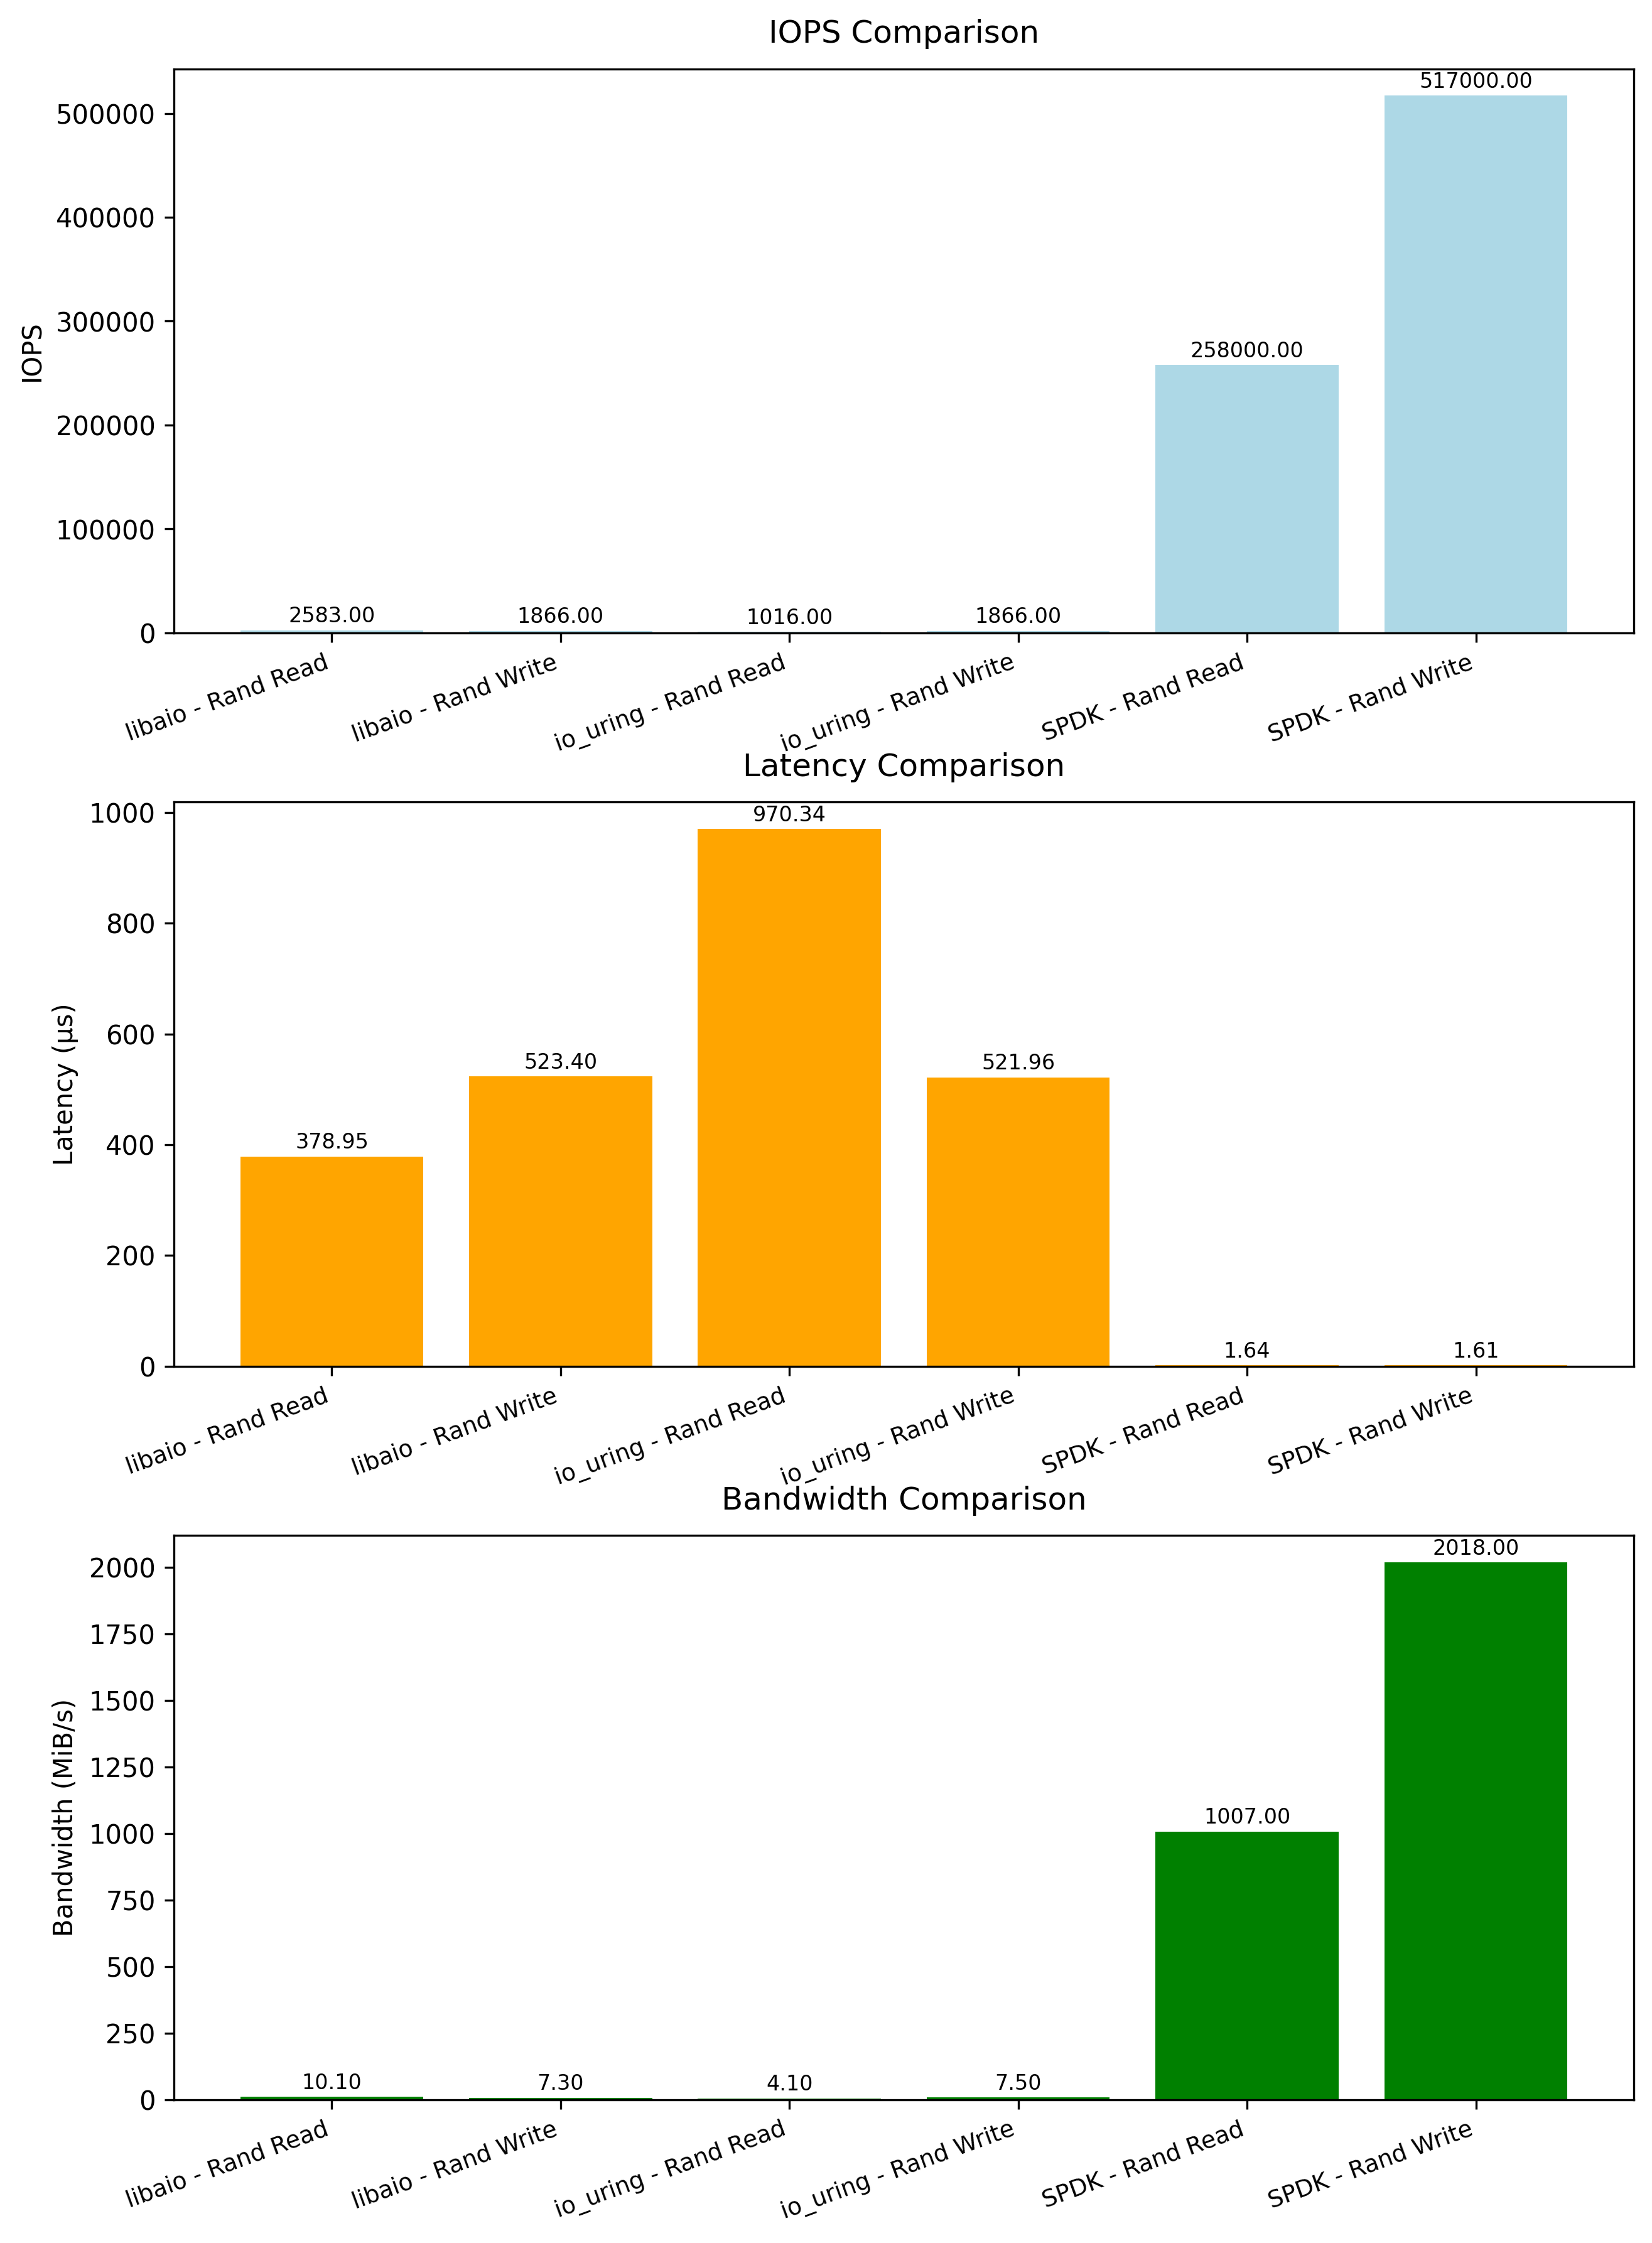
\includegraphics[width=\textwidth]{figs/Overview.png}
‫    \caption{مقایسه‌ی کلی}
‫\end{figure}
‫
‫
‫\begin{figure}[H]
‫    \centering
‫    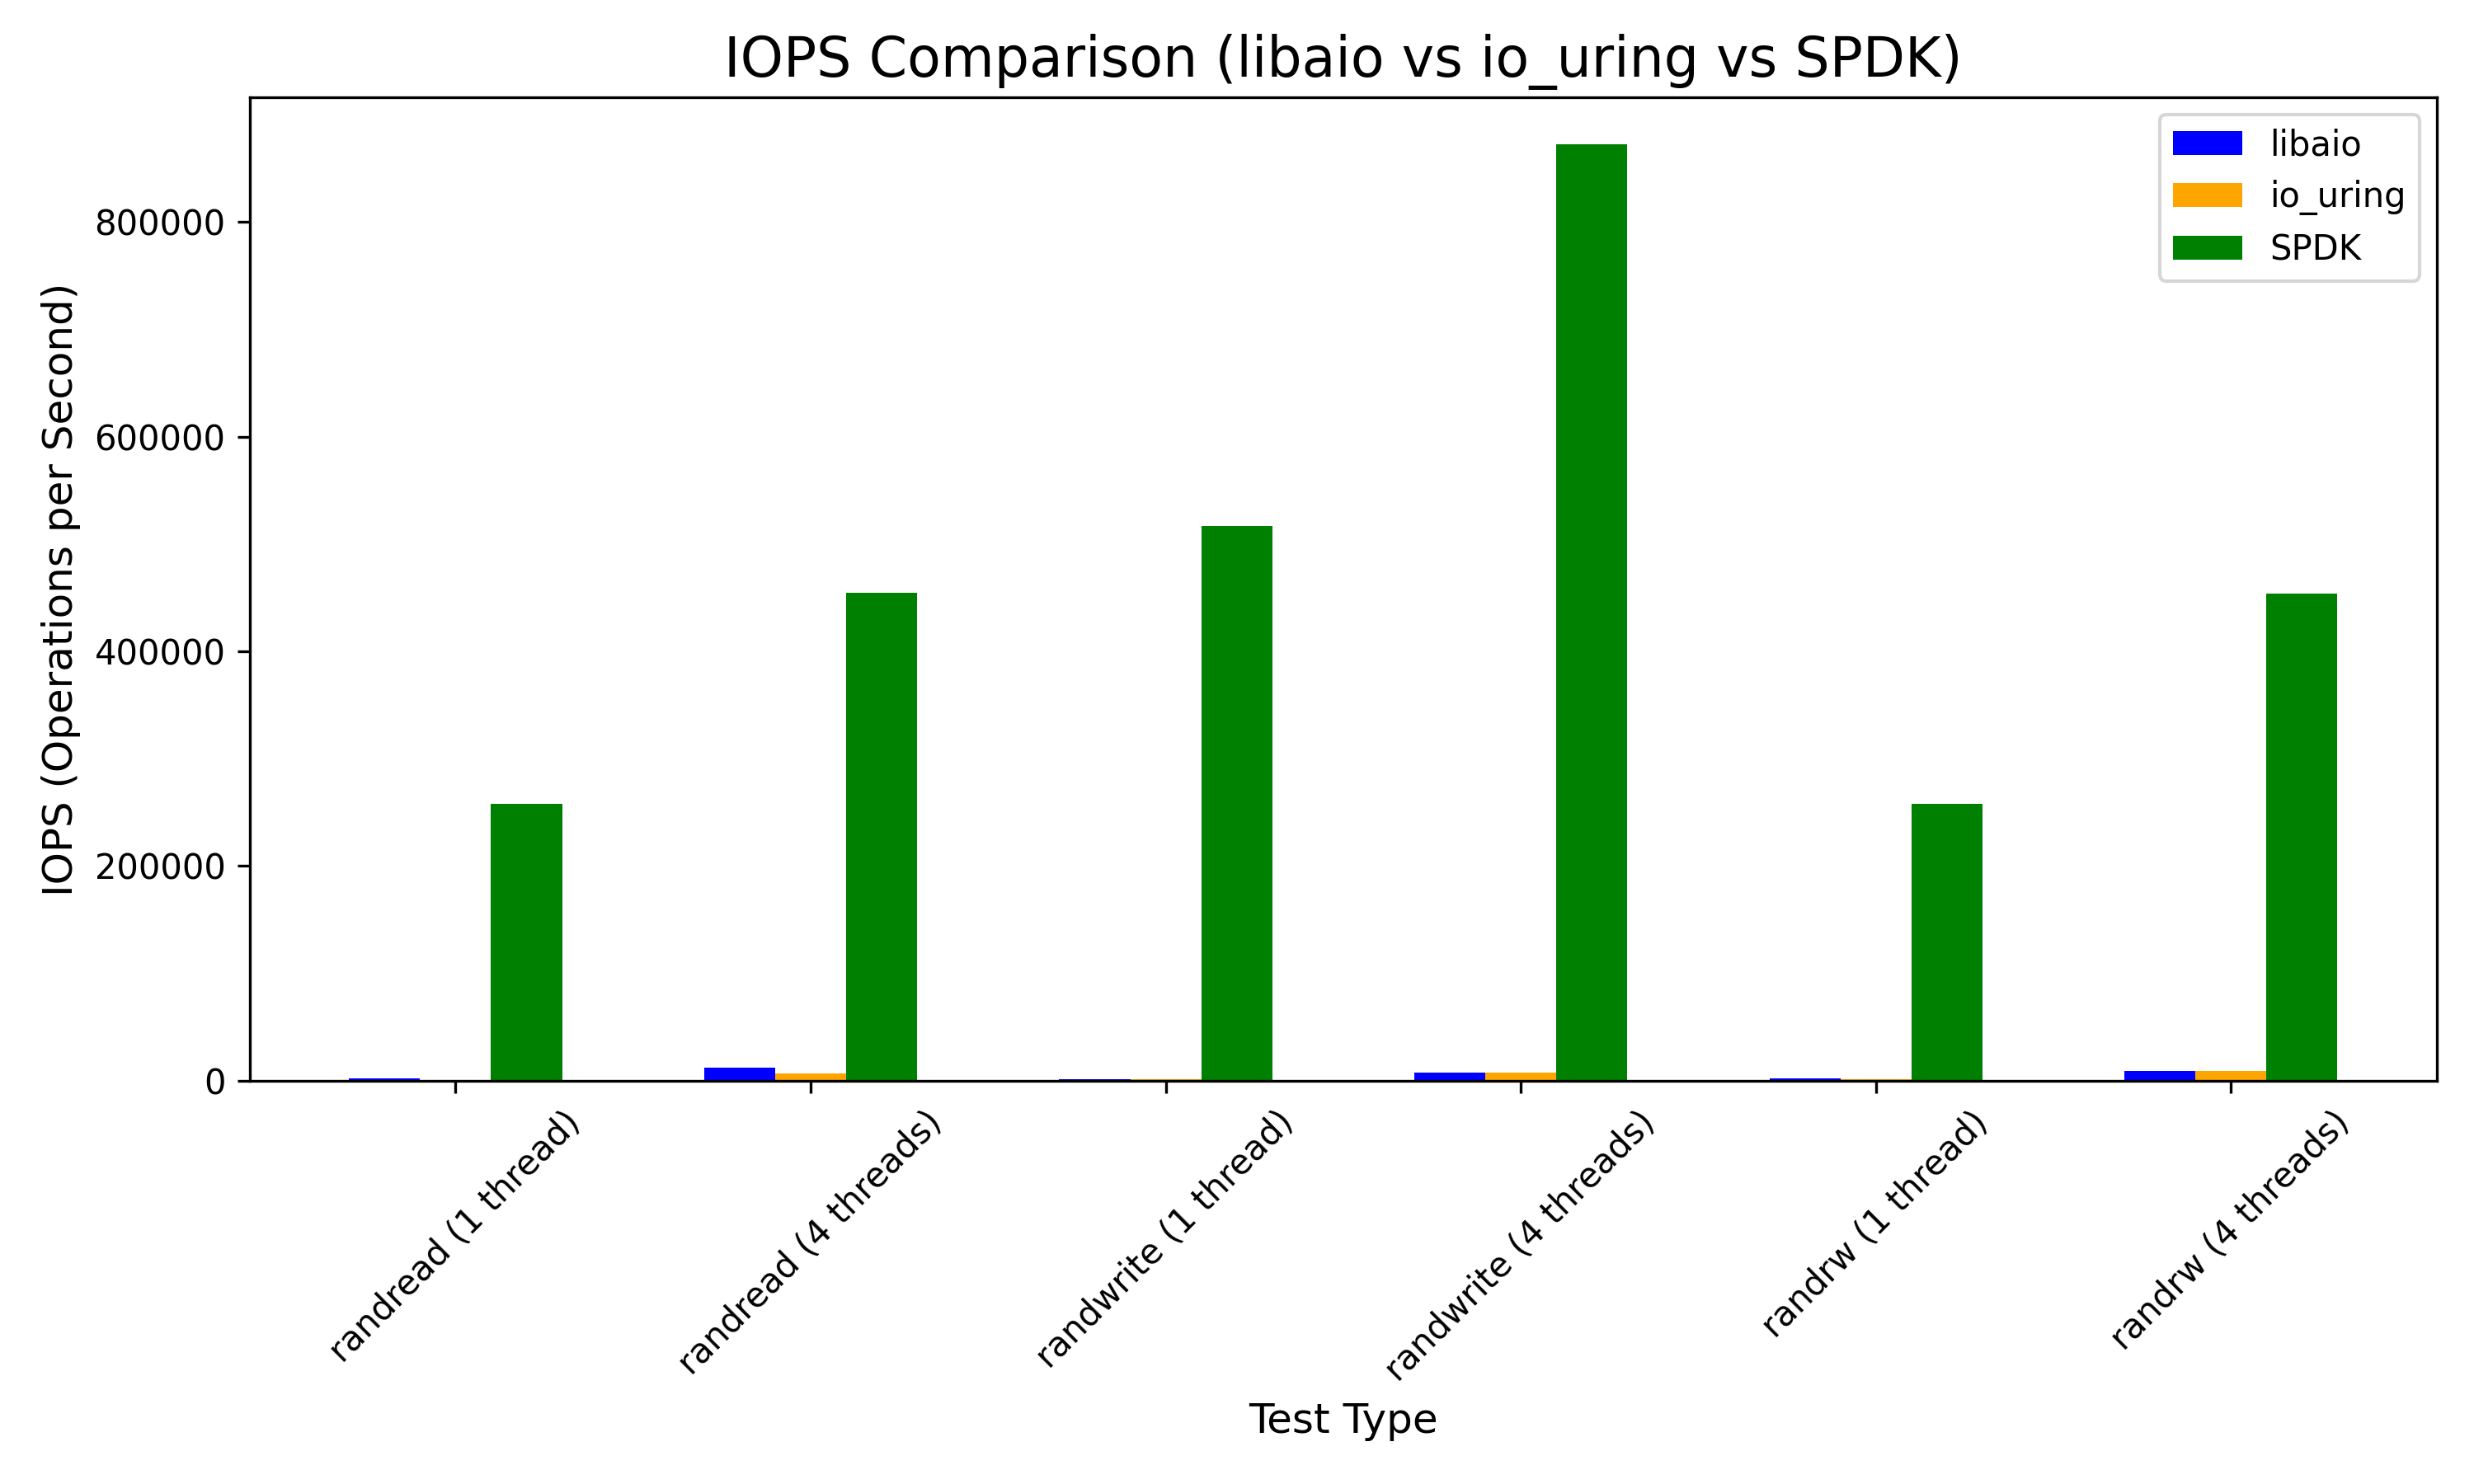
\includegraphics[width=\textwidth]{figs/iops_comparison.png}
‫    \caption{مقایسه‌ی IOPS}
‫\end{figure}
‫
‫
‫\begin{figure}[H]
‫    \centering
‫    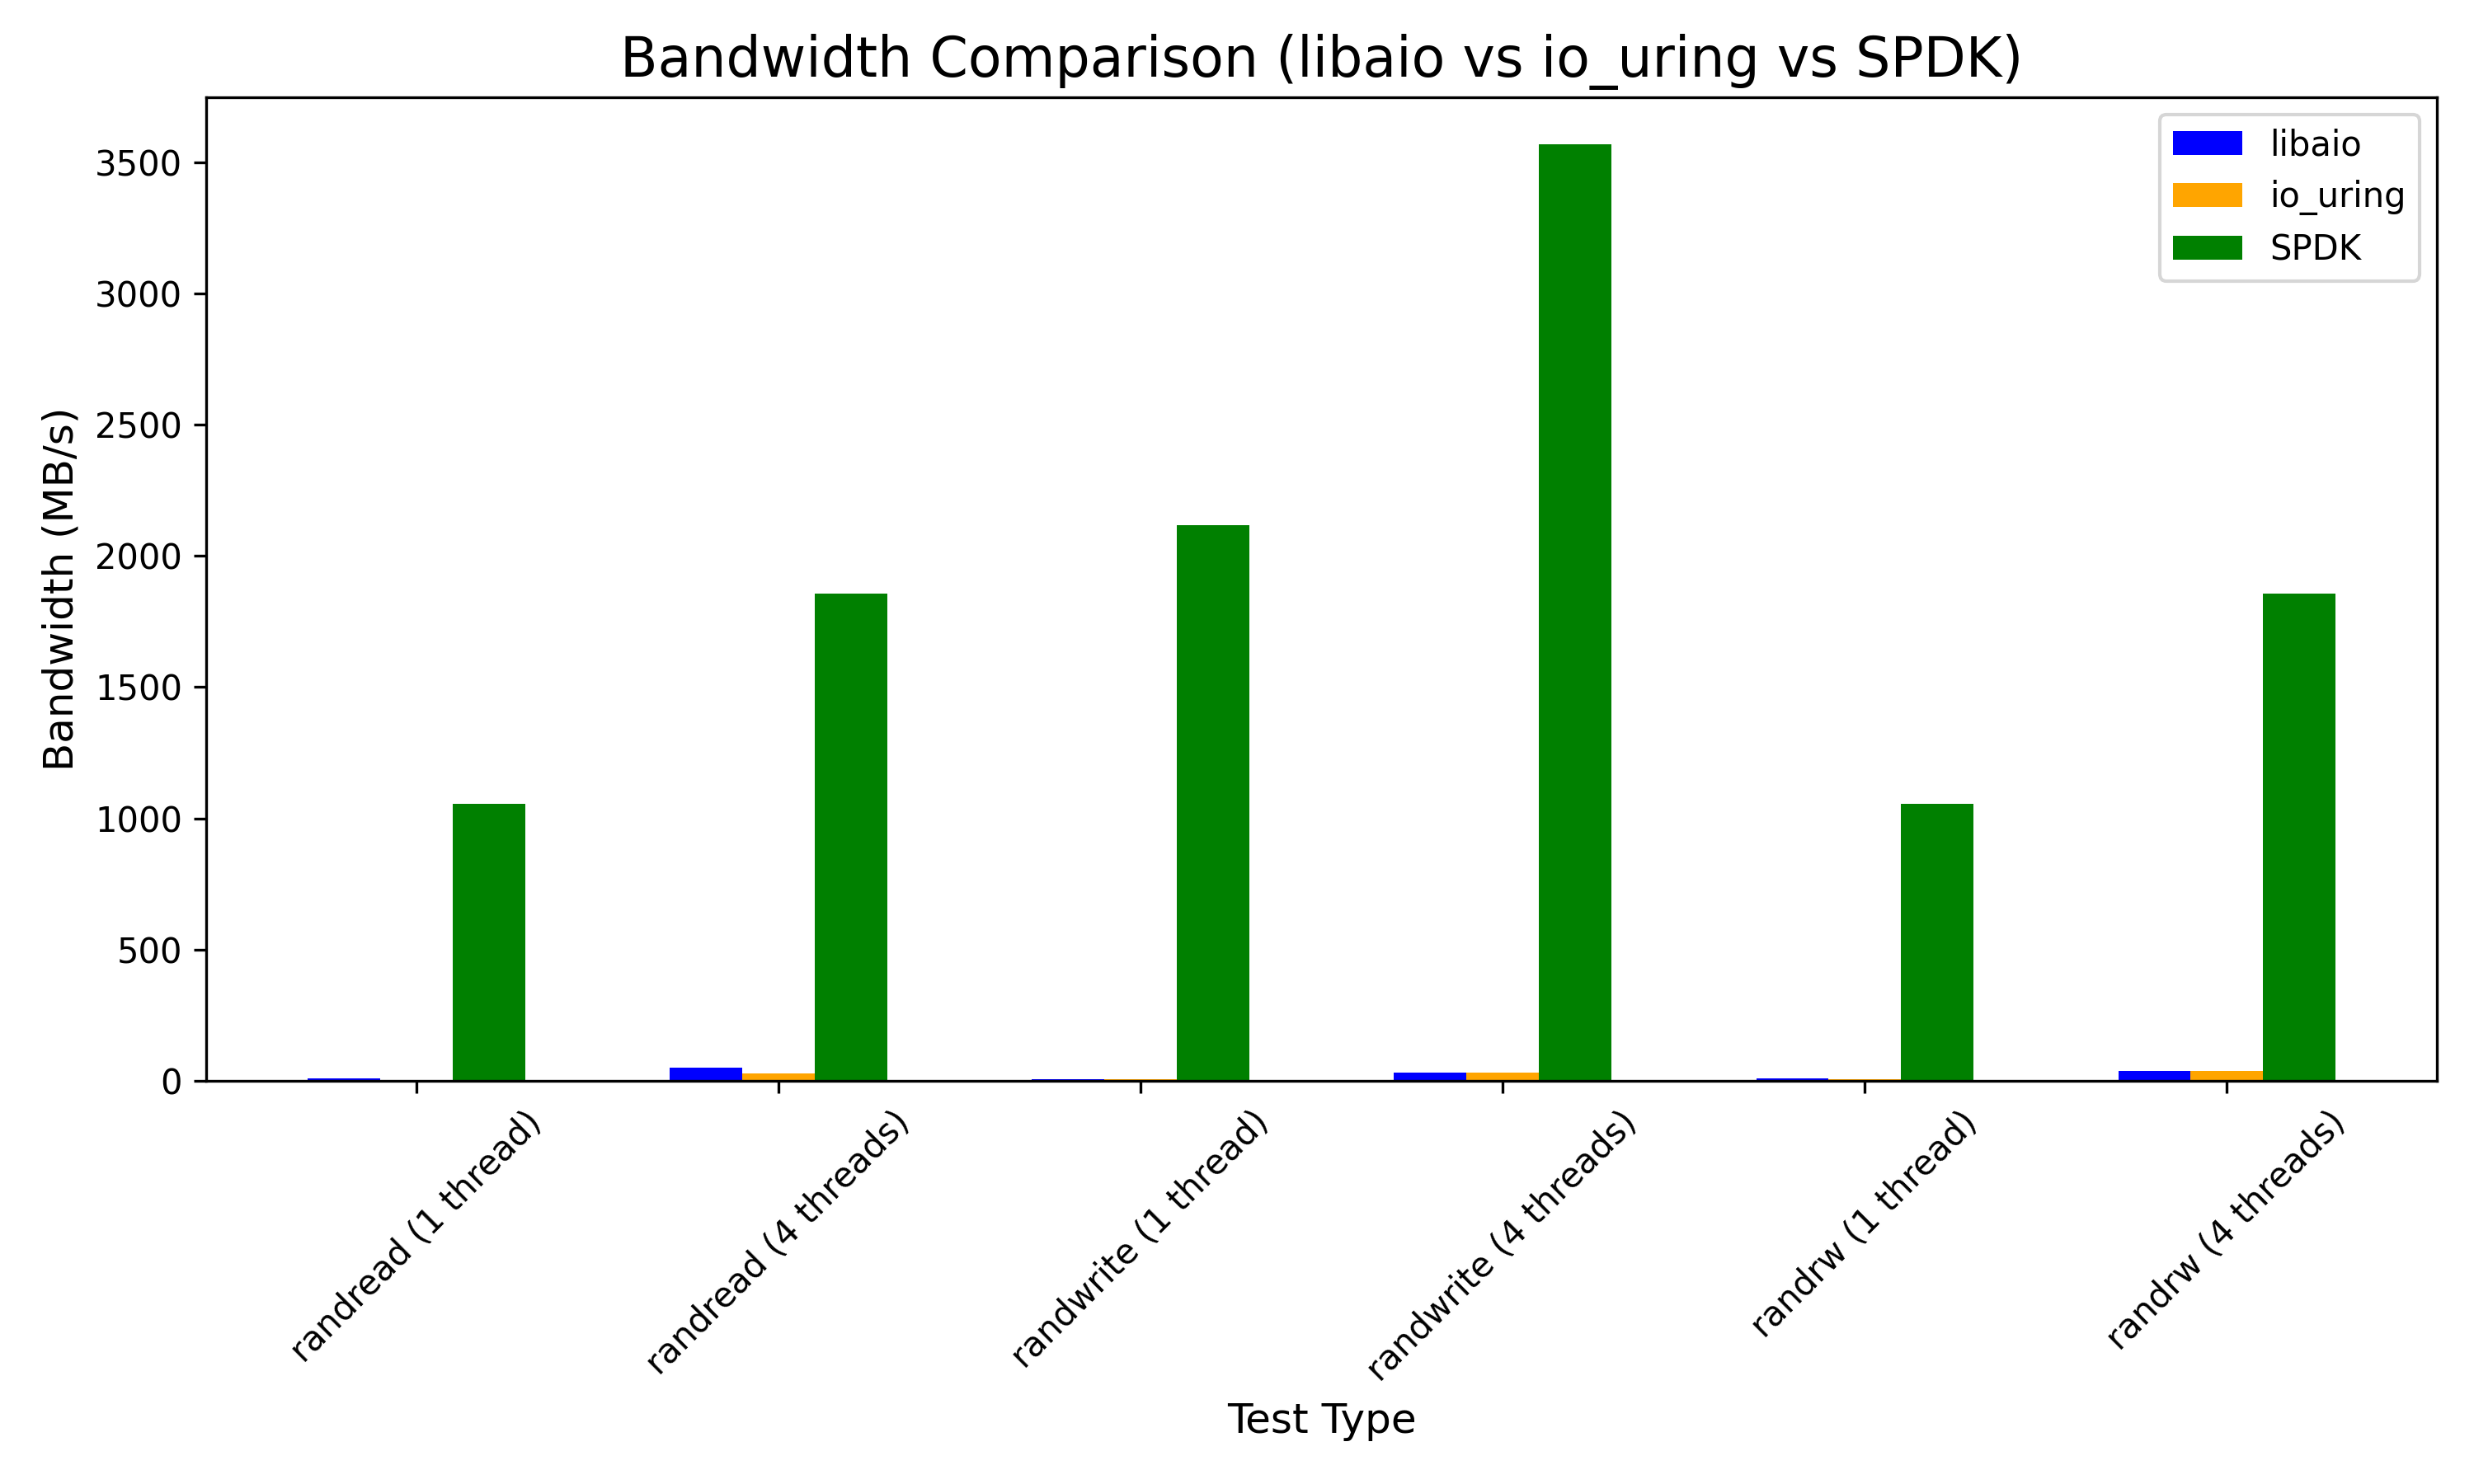
\includegraphics[width=\textwidth]{figs/bandwidth_comparison.png}
‫    \caption{مقایسه‌ی Bandwidth}
‫\end{figure}
‫
‫
‫\begin{figure}[H]
‫    \centering
‫    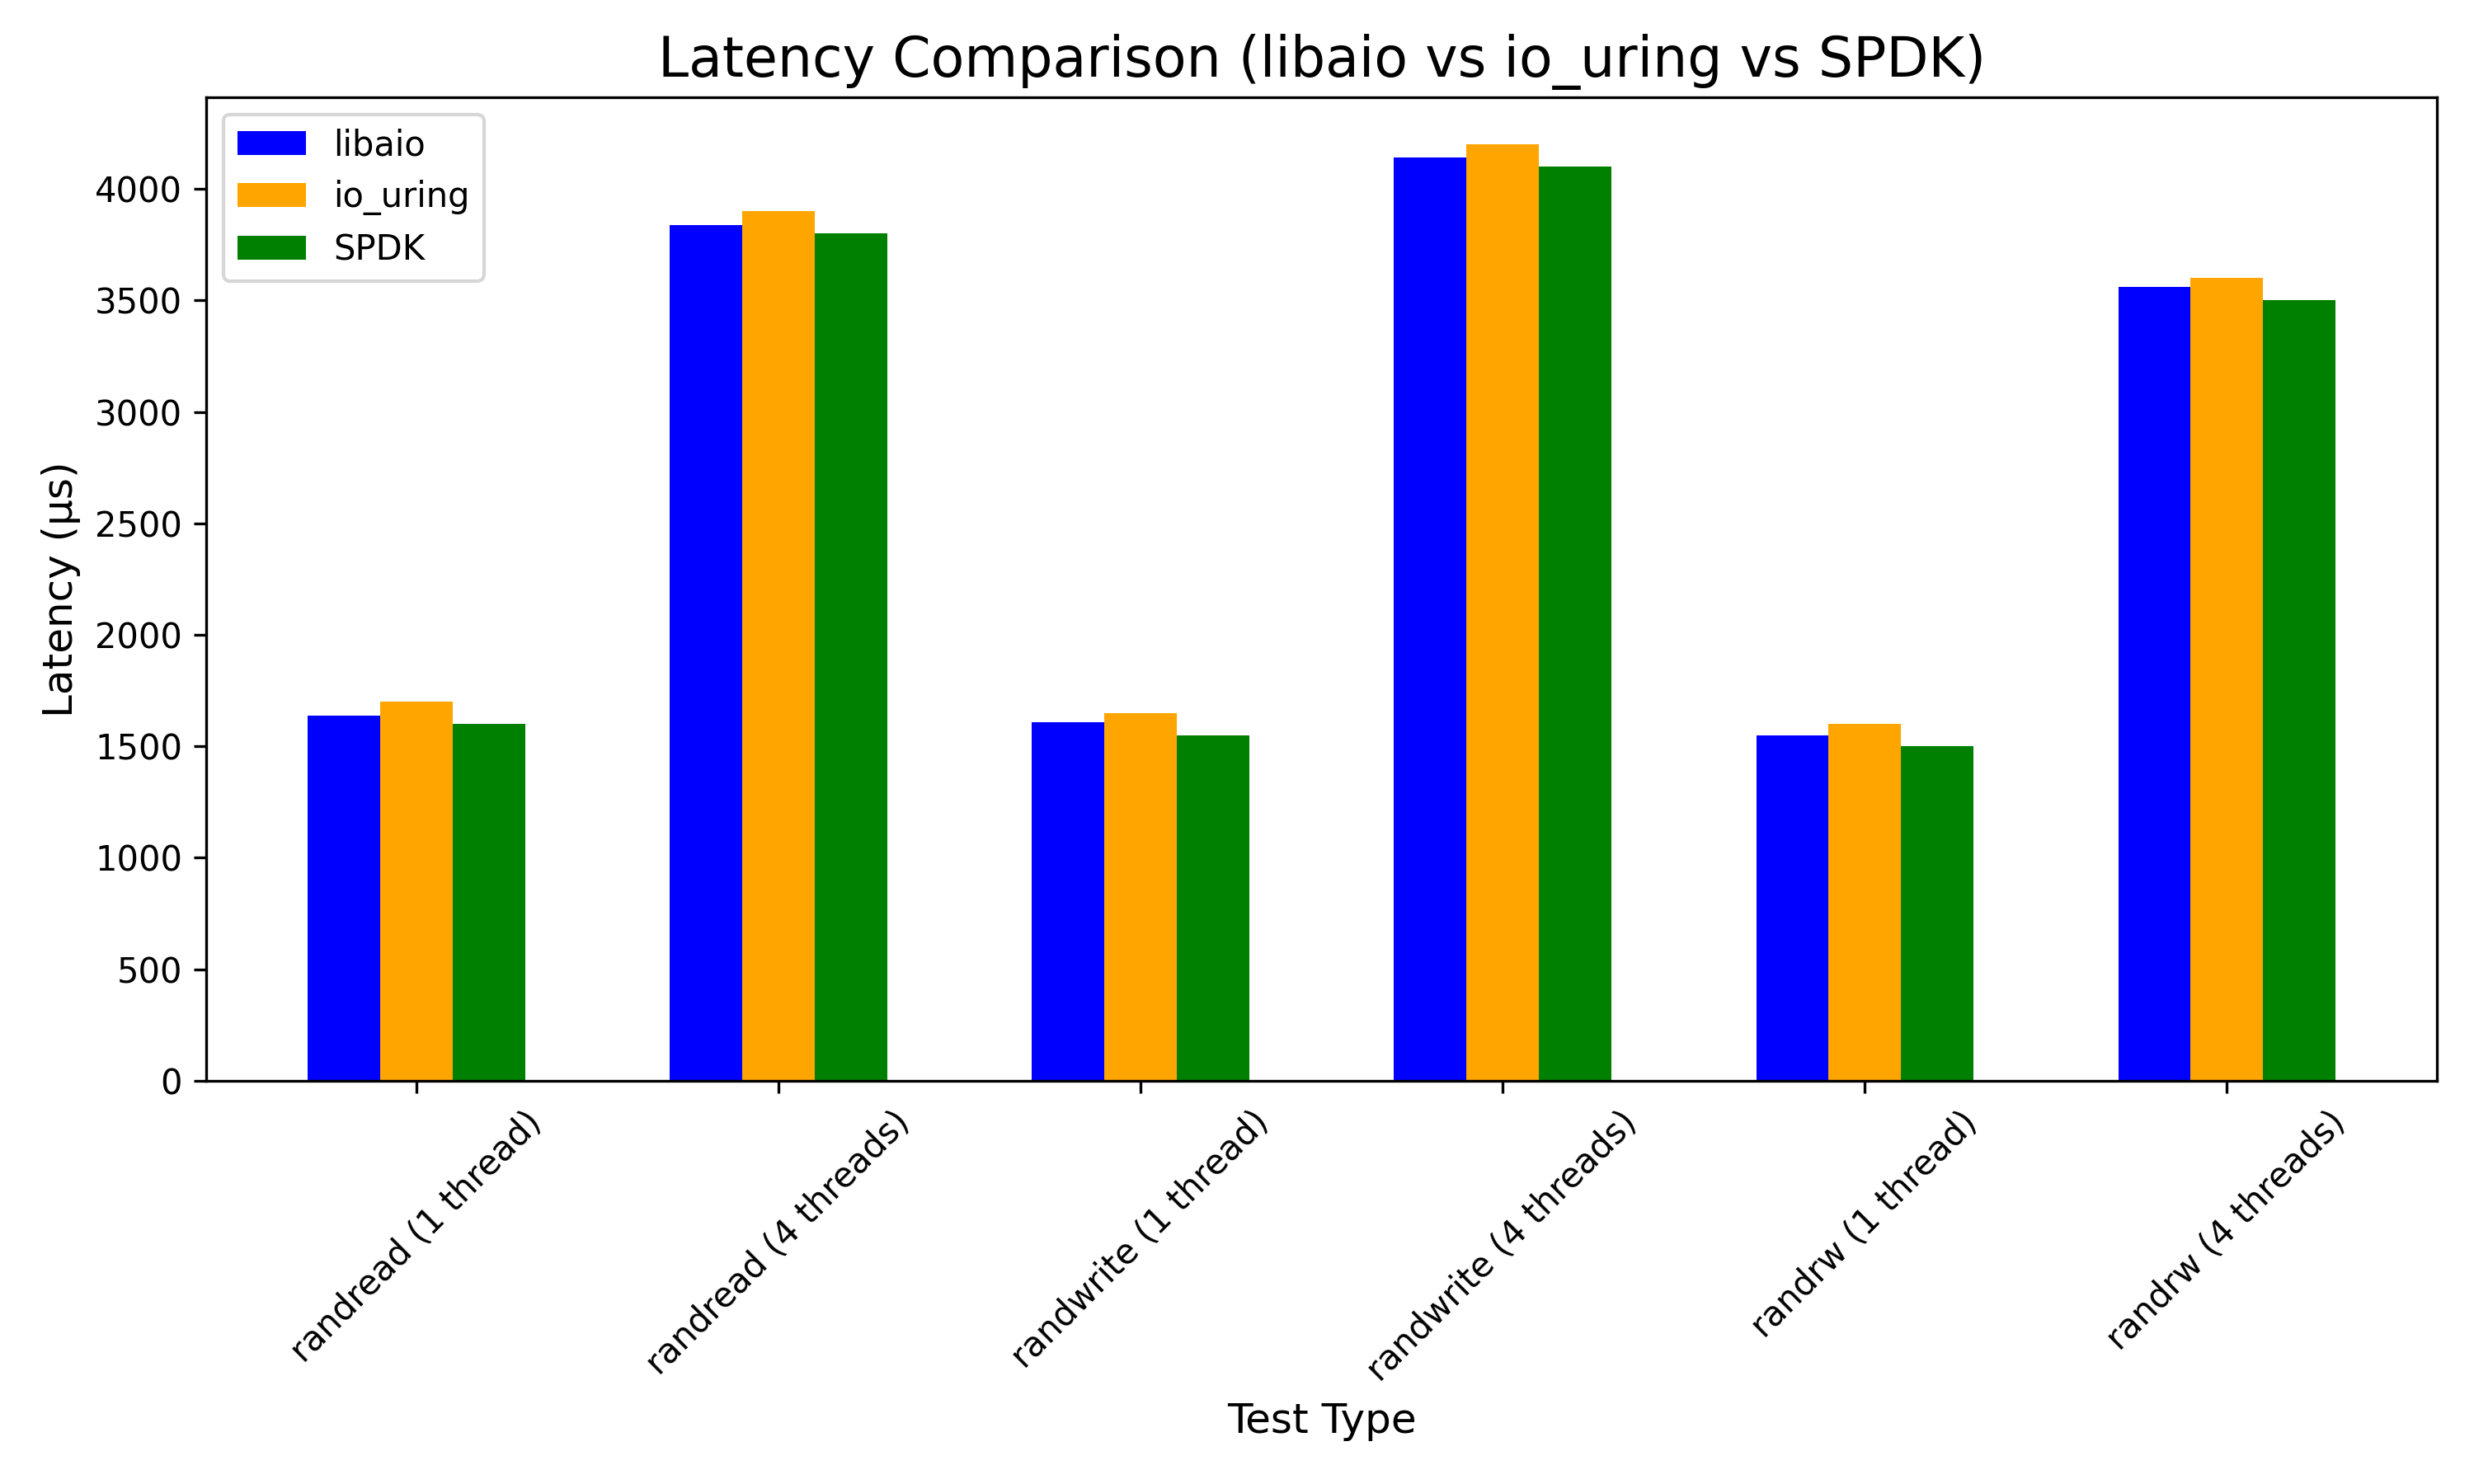
\includegraphics[width=\textwidth]{figs/latency_comparison.png}
‫    \caption{مقایسه‌ی Latency}
‫\end{figure}
‫
‫\پایان{لوح}
‫
‫